\chapter[The Waterfall Target]{The Waterfall Target
\footnote{
  $CVS~revision~ $Id: waterfall-target.tex,v 1.6 2003/12/13 06:23:39 gen Exp $ $
}
\footnote{Authors: David Meekins \email{meekins@jlab.org} and 
 Maurizio Lucentini \email{lucentin@jlab.org}. \\
 This file is a combination of two files taken from: \\
 \url{http://www.jlab.org/~meekins/h20_target/safety_doc/},\\
  \mycomp{Operation\_manual.lyx} and \mycomp{waterfall\_safety.lyx}.
  The original documents are available:\\
 \url{http://www.jlab.org/~meekins/h20_target/safety_doc/Operation_manual.ps} and\\
 \url{http://www.jlab.org/~meekins/h20_target/safety_doc/waterfall_safety.ps}\\
 The file has been formatted by J.LeRose \email{lerose@jlab.org}
 and E.Chudakov \email{gen@jlab.org}
}}
% \newcommand{\boldsymbol}[1]{\mbox{\boldmath $#1$}}

\section{Overview}
\label{sec:wt_overview}

The waterfall target system provides a target for experiments on 
$^{16}$O. Using a waterfall for oxygen experiments has many advantages. Pure 
oxygen is difficult to handle, as it is highly reactive. The use of other 
oxygen compounds requires additional measurements to subtract the non-oxygen 
background, whereas the hydrogen in water can be used for calibration purposes.
The technique of using continuously flowing water as an electron scattering 
target was first developed in 1982 in Mainz~\cite{Voegler:1982}.
The conceptual design of the waterfall target system for Hall A
developed by INFN Roma, 
is very similar to one used at Saclay~\cite{Garibaldi:1992mb},
with the parameters as follows: ~$\sim 120$~mg/cm$^{2}$ one-foil thickness,
target thickness stable in time within 1\%, and insensitive
to beam current up to at least 20~$\mu$A.
The target may be configured for one or multiple waterfall 
``foils''. 


\section{Description of the System}
\label{sec:wt_descrip_sys}

The main components of the target system (see Fig.~\ref{fig:wt_uno}
 \infolevtwo{and Fig.~\ref{fig:wt_uno-mau}}%infolev 
) are: 
\begin{list}{}{\setlength{\itemsep}{-0.15cm}}
\item[a)] the waterfall target cell, the target, the solid target ladder; 
\item[b)] the hydraulic system; 
\item[c)] the movement system; 
\item[d)] the slow-control system; 
\end{list}

\begin{figure}[htp]
\begin{center}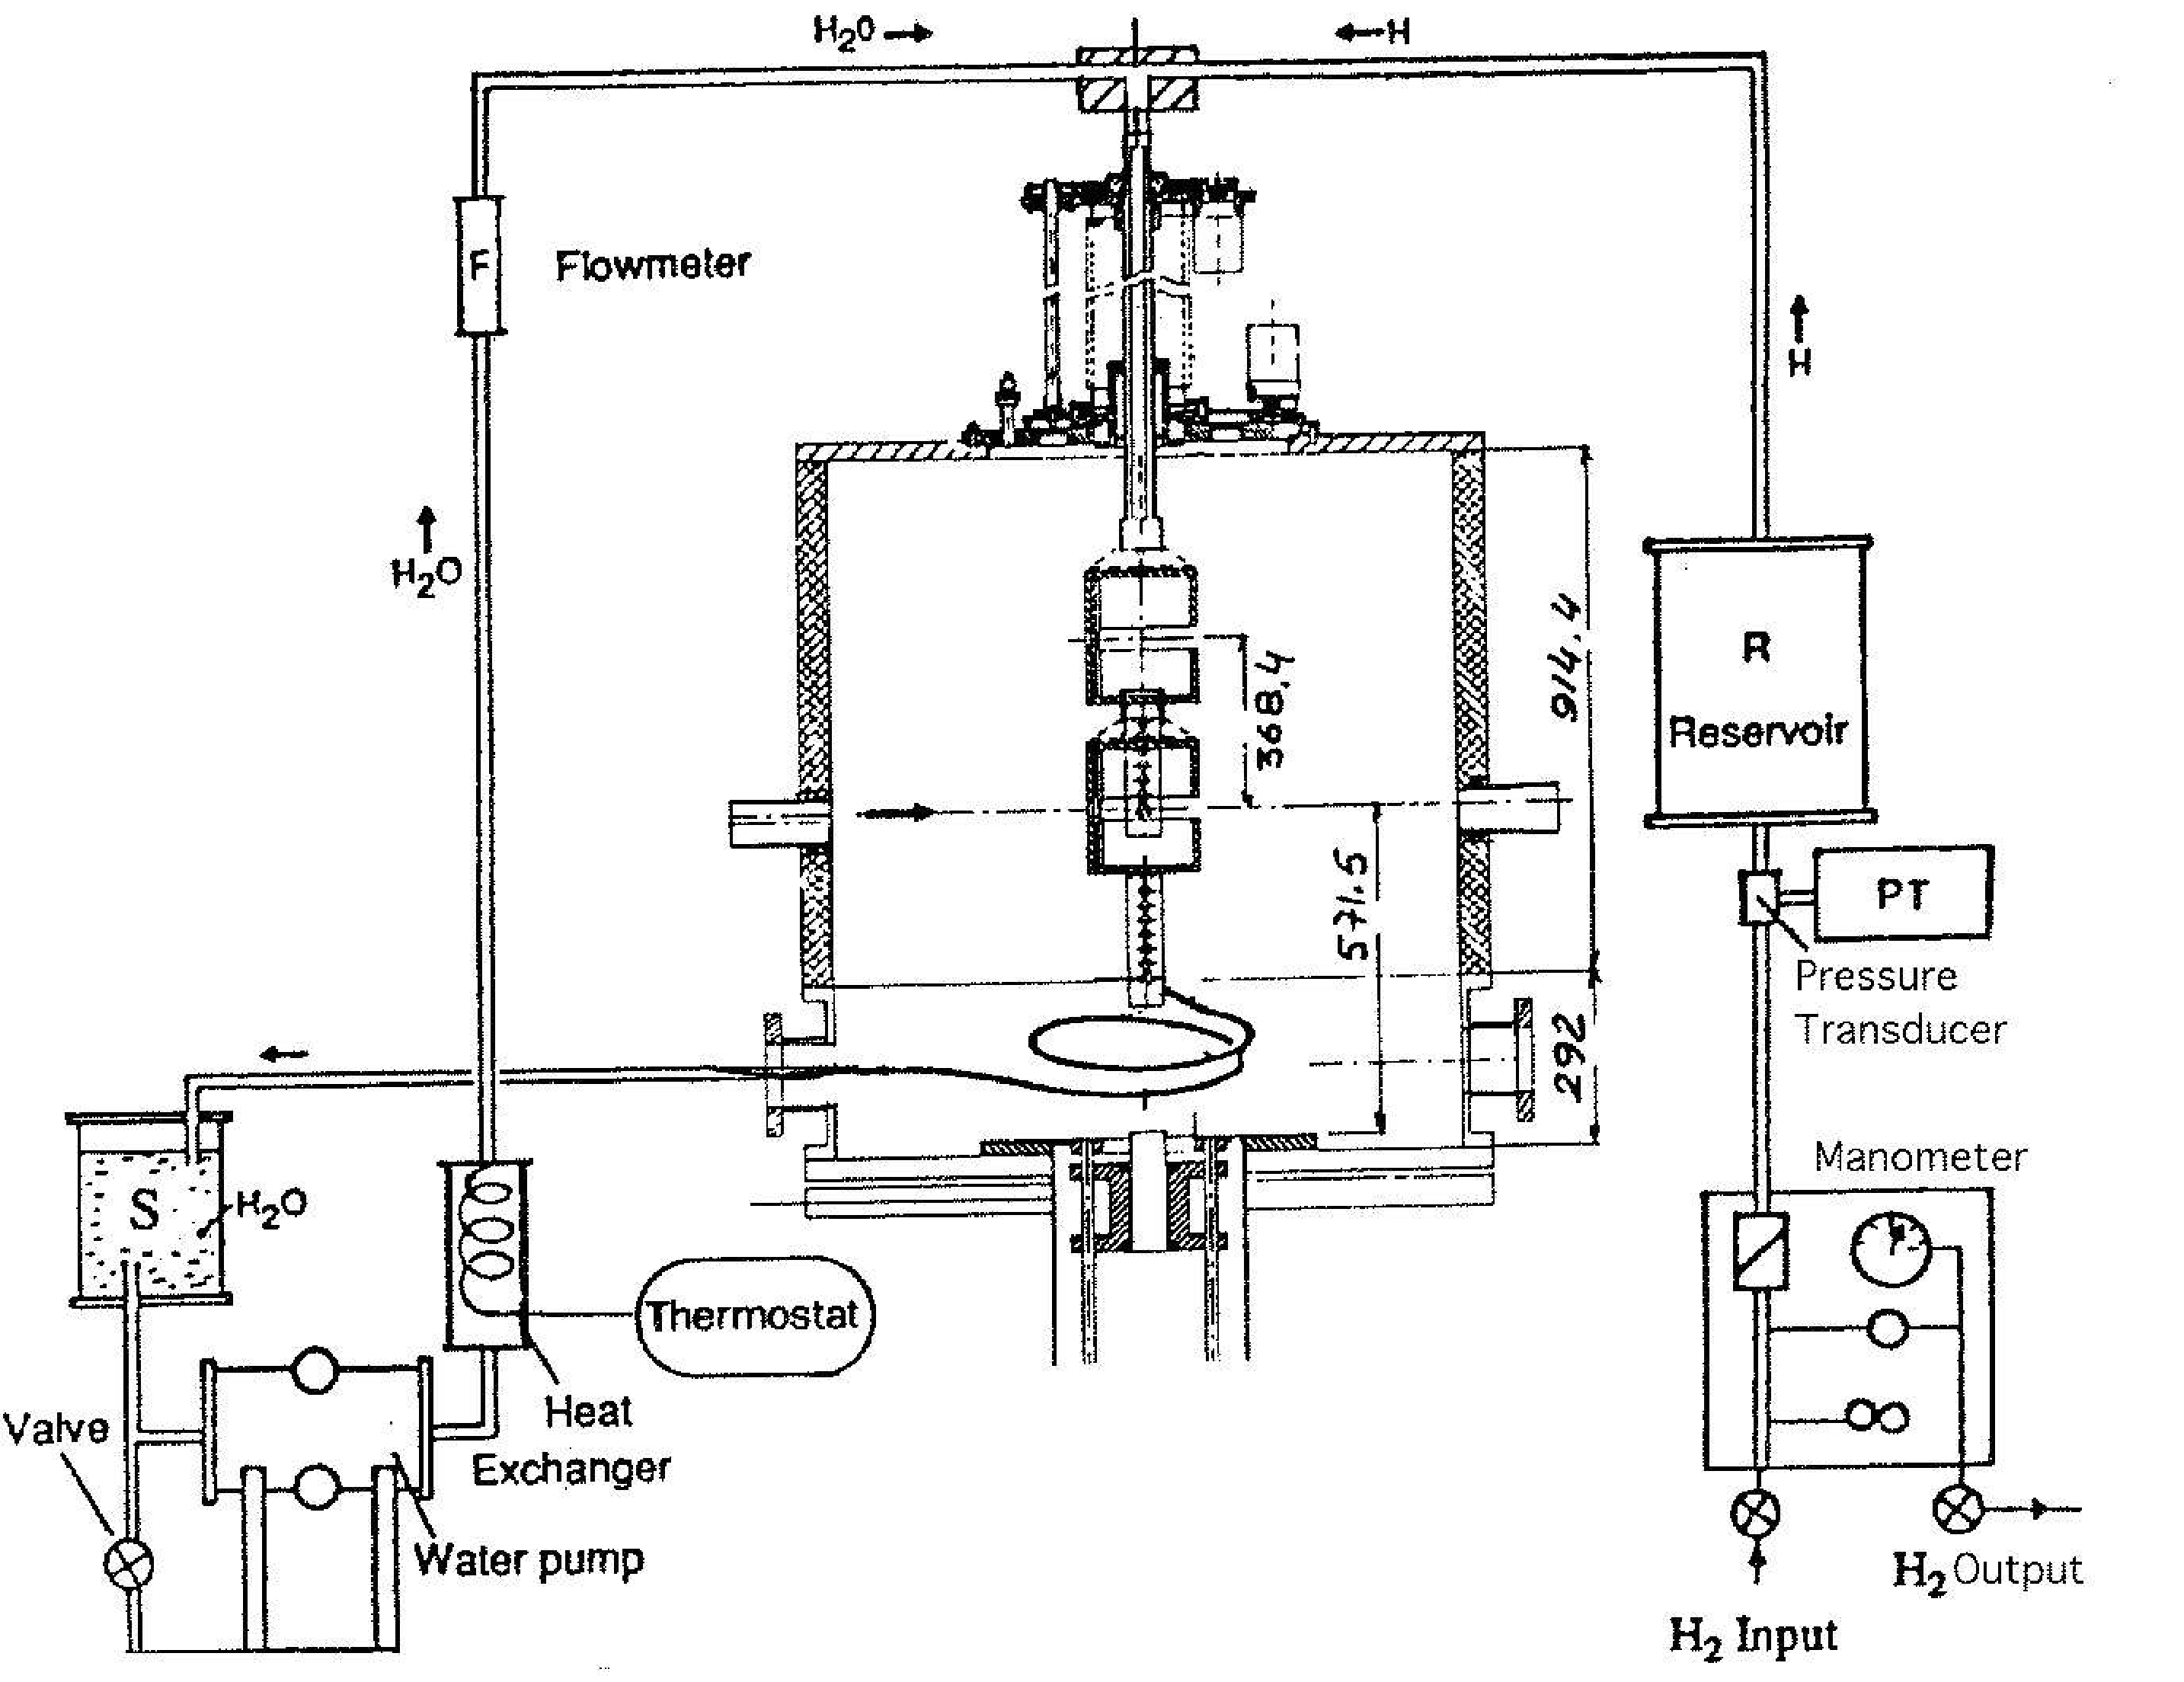
\includegraphics[  width=0.9\textwidth]{wt2_uno_OLD}\end{center}
\caption[Waterfall target system]%
{Schematic overview of the target system with the hydraulic system
  on the left side, scattering chamber, movement system and target cell
  in the middle. The hydrogen system on the right side is not implemented
  in the present setup.}
\label{fig:wt_uno}
\end{figure}

%
\infolevtwo{
  \begin{figure}
  \begin{center}
     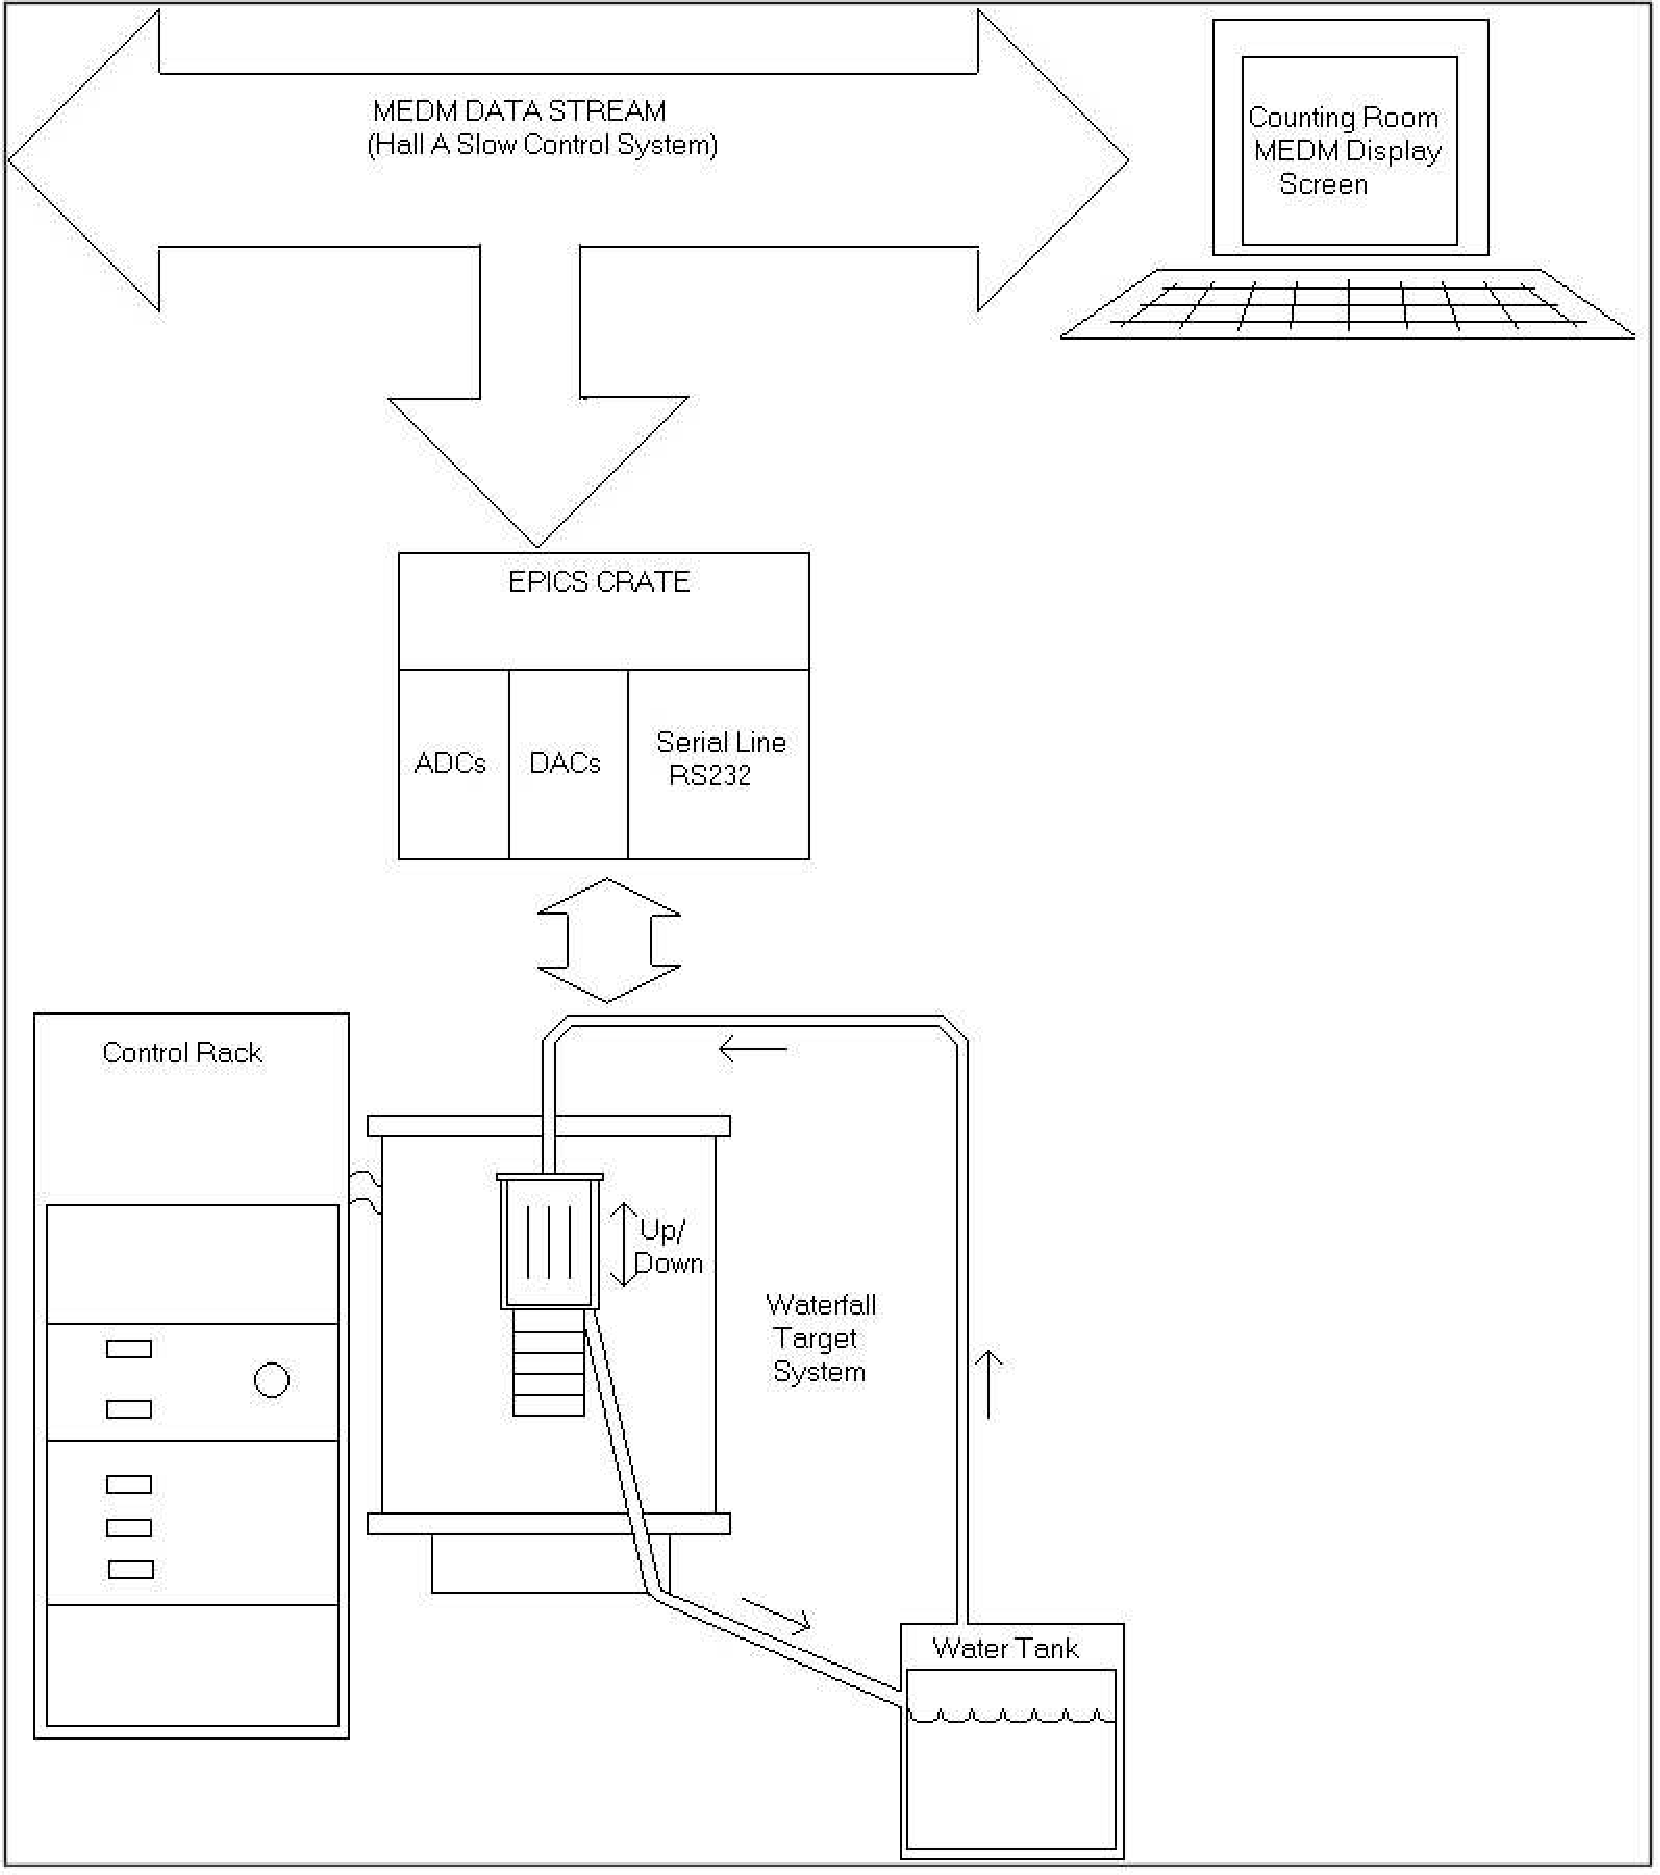
\includegraphics[width=\textwidth]{wt2_uno-mau}
  \end{center}
  \caption{Scheme of the target system devices}
  \label{fig:wt_uno-mau}
  \end{figure}
}%infolev

The waterfall foil(s) is (are) produced in a cell mounted in the standard
scattering chamber 
\infolevfour{
 (Fig.~\ref{fig:wt_tposi} and \ref{fig:wt_enclosure})
}%infolev
of Hall A. 
The water, continuously pumped from a reservoir~(S), goes into
the target cell and then back into the reservoir. The water passes
through a system of slits and holes to form one or more flat rectangular
films, which are stable due to the surface tension and to the adherence
to stainless steel poles% 
\infolevfour{ (Fig.~\ref{fig:wt_thfoil})}.%infolev
Under the cell, a
target holder allows one to put up to 5 solid targets cooled by the
water% 
\infolevfour{ (Fig.~\ref{fig:wt_target-stack})}.%infolev

The waterfall target can consist of a single foil or multiple foils,
according to the needs of the particular experiment. Notice that it
is possible to modulate, slightly, the thickness of the waterfall
target by changing the pump speed. This adds flexibility to the system
and allows the user to choose the best value according to the desired
resolution and luminosity.

Elastic scattering from hydrogen in the target is used to measure
the target thickness. For continuous monitoring of the target thickness,
one `calibrates' the raw counting rate of either spectrometer by the
elastic scattering measurement. It is then possible to convert the
electron or hadron rate observed during the measurement to an average
target thickness.

\infolevltone{
For more information consult the full OSP manual~\cite{HallAosp}.
}%infolev

\infolevfour{

\begin{figure}[htp]
%\begin{center}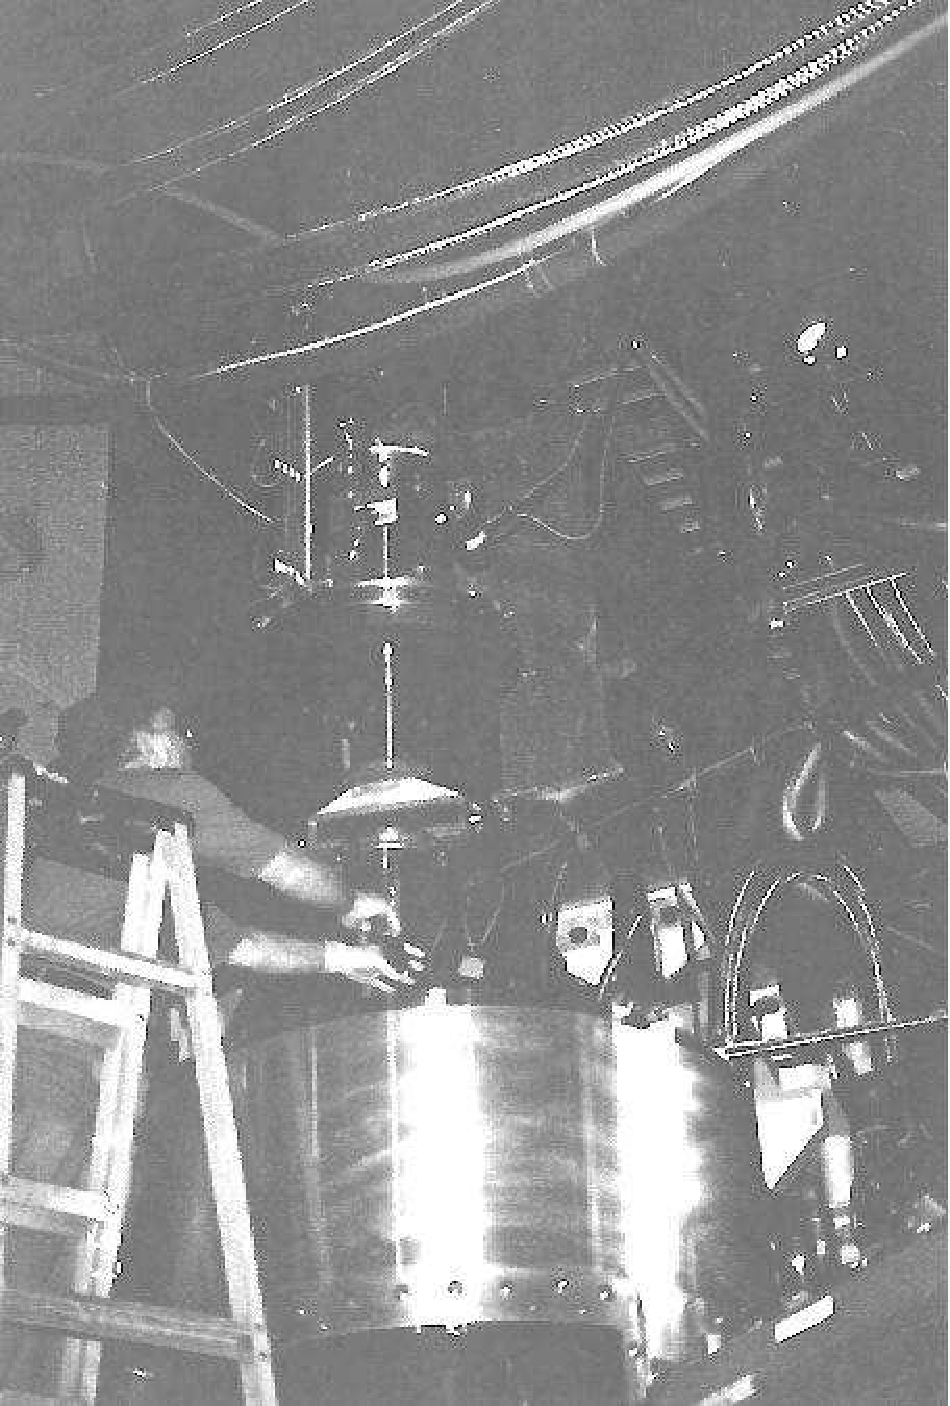
\includegraphics[width=8cm]{wt2_targetpositioning_bw}\end{center}
\begin{center}
  \includegraphics*[height=0.4\textheight]{wt2_targetpositioning_bw}\hfill
  \includegraphics*[height=0.4\textheight]{wt2_scatt_chamb}
\end{center}
\caption{Pictures of the target and scattering chamber.}
\label{fig:wt_tposi}
\end{figure}
%
\begin{figure}[htp]
%\begin{center}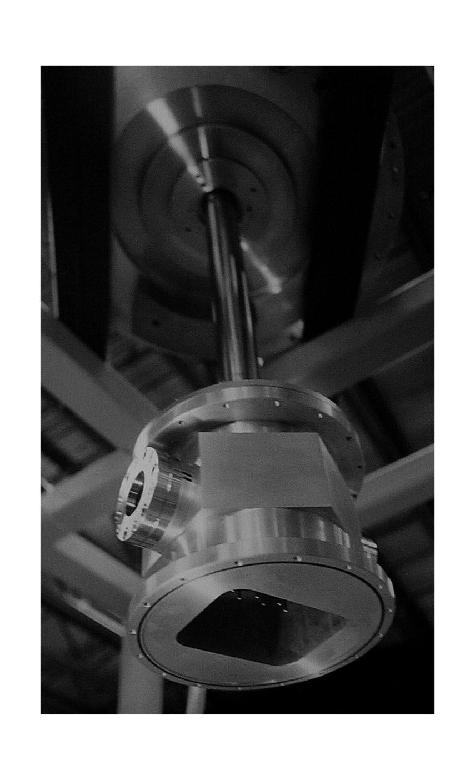
\includegraphics[  width=10cm]{wt2_enclosure}\end{center}
\includegraphics*[height=0.4\textheight]{wt2_enclosure}\hfill
\includegraphics*[height=0.4\textheight]{wt2_targ_encl}
\caption[The enclosure of the target used for E00-102 and E94-107]%
{The enclosure of the target used for E00-102 and E94-107 
        is shown on the left. The waterfall target within the enclosur
        is shown on the right.}
\label{fig:wt_enclosure}
\end{figure}
%
\begin{figure}[htp]
\begin{center}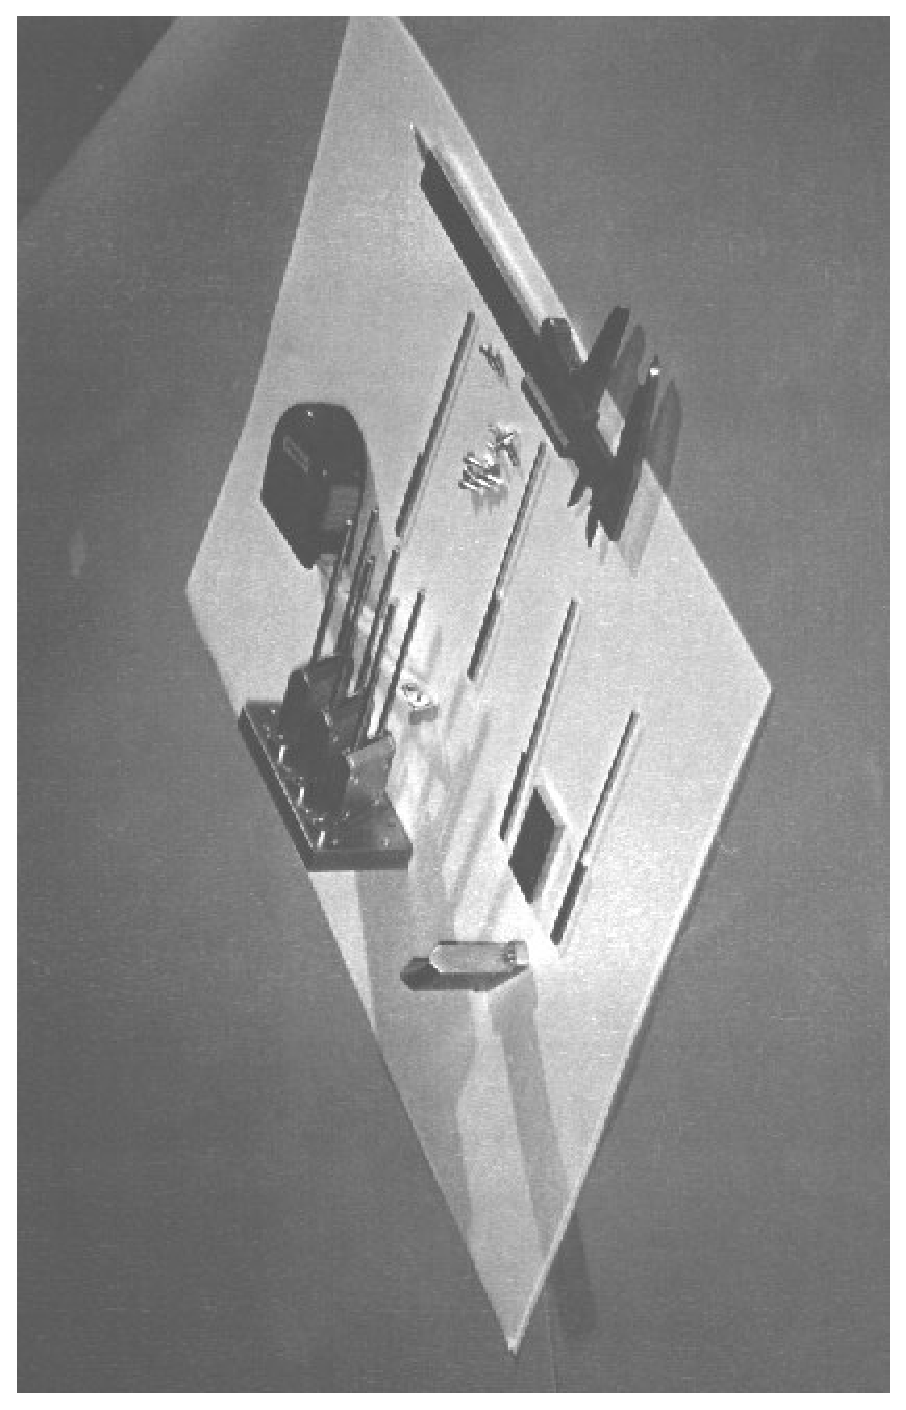
\includegraphics[angle=-90,width=0.7\textwidth]{wt2_threefoils_bw}\end{center}
\caption{Mechanical details of the waterfall target: posts etc.}
\label{fig:wt_thfoil}
\end{figure}

\begin{figure}
\begin{center}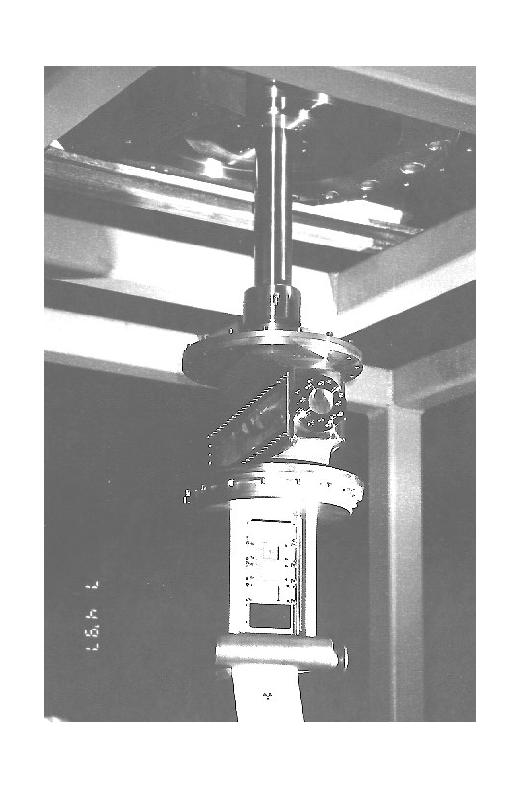
\includegraphics[  width=0.90\textwidth]{wt2_target_bw}\end{center}
\caption[The Waterfall Target Stack]%
{The Waterfall Target Stack, the waterfall cell with solid targets 
         mounted beneath\label{fig:wt_target-stack}.}
\end{figure}
} %infolev

\infolevone{

\subsection{The Hydraulic System}

The hydraulic system comprises of a closed circuit (Fig.~\ref{fig:wt_acqua})
containing a pump which forces the water from a stainless steel container
up to the target manifold and back to the container by means of stainless
steel tubes. A gear pump, magnetically coupled to a dc motor, is used
to produce a stable film.

\begin{figure}
\begin{center}
   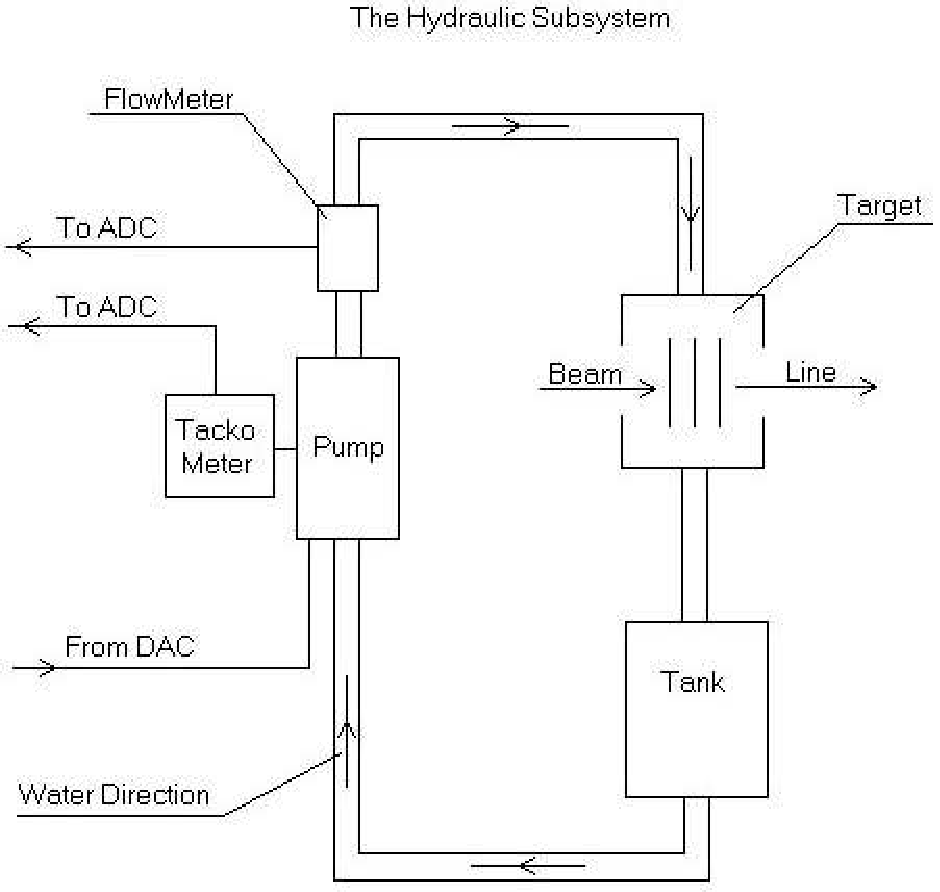
\includegraphics[height=0.8\textheight,width=0.9\textwidth]{wt2_hydr_sub}
\end{center}
\caption{Schematic view of the hydraulic system.}
\label{fig:wt_acqua}
\end{figure}


There is a provision to place a cooler along the circuit to keep the
water at constant temperature. Moreover, hydrogen can be introduced
into the target container to reduce the background. In the present
setup, neither of these provisions have been implemented.

A tachometer on the pump axis measures the pump speed (RPM) and a
flowmeter, just before the entrance of the scattering chamber, measures
the flow rate. The command voltage value is also read. By continuously
measuring these parameters, and comparing them, one can monitor the
target thickness stability.

Basically, the water flows in a closed loop; there is a magnetic gear
pump, capable of 40 liters/min, 0-90~V DC voltage controlled, which
pulls the water in a stainless steel tube, from the rack up to the
target cell, at a distance of about 20 metres. Before arriving in
the cell, the water flows through a flowmeter. A display shows the
flux in front of the rack.

When the water arrives at the target cell, it passes through a small
compression chamber, which has three rectangular holes at its bottom.
Three waterfalls are formed. Finally, the water falls down the cell
where an output stainless steel tube goes back to the tank%
\footnote{The tank is a parallelepipedal volume of about 20 liters made of stainless
steel with a front perspex window, which can be seen in front of the
rack, to see the inner water level.%
}. When the pump is off, the water nearly fills the tank. When the
pump is on, the water level must be sufficient to let the pump pull
water, and not air. The pump speed is read by a tachometer, which
consists of an optical counter-timer which counts the turns of the
pump axis, and sends this value to a display in front of the rack
and to the computer by a 4-20~mA standard loop.

The pump has a driver located on top front of the rack, which allows
the user to drive it manually, or from a remote position using the
computer. A manual switch on the front of the driver selects the operating
mode. If manual mode is set, the knob close to the switch can be turned
in order to increase/decrease the pump speed. The value of the pump
speed represents the percentage of maximum reachable pump speed (see
Operating Procedure). The pump speed regulator is also available in
the Counting Room. The pump cannot be switched off by computer. \\


A short list of the instruments used in this systems is listed below: 

\begin{center}\begin{tabular}{ll}
\hline 
Device &
 Model \\
\hline
Flowmeter probe &
 \\
 Flowmeter transducer and transmitter &
 NA\\
 Flowmeter display &
 ITECO trading mod. 9210001 out 4-20~mA \\
 Tachometer &
 ITECO trading mod. 9210001 out 4-20~mA \\
 Water pump &
 Pacific Scientific mod. 6324-452 \\
 Pump driver &
 Dart Controls mod.253G 200E + PCM23 \\
 Tubes &
 Swagelock tubes (various sizes) \\
 Tube Connectors &
 Swagelock tube connectors  \\
\hline
\end{tabular}\end{center}

} %infolev

\infolevone{

\subsection{The Movement System}

The movement system allows the vertical translation of the waterfall
target and the solid target ladder. The total mass of the system is
about 50~kg.
\infolevfour{
  A picture of it can be seen in Fig.~\ref{fig:wt_total-view}.
  \begin{figure}
  \begin{center}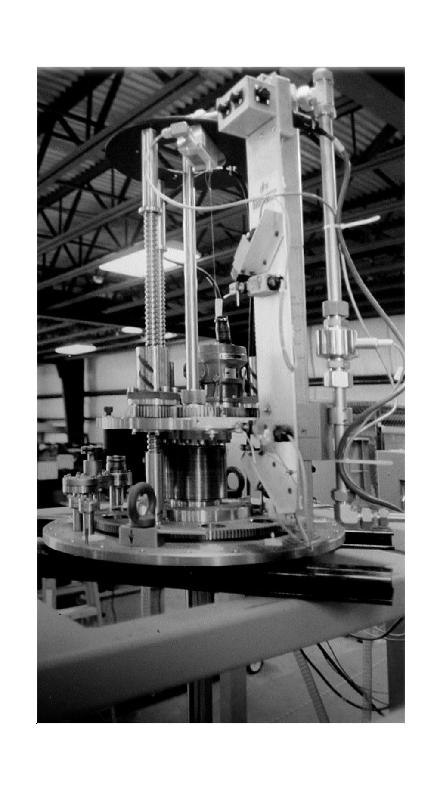
\includegraphics[height=0.8\textheight]{wt2_view_of_syst}\end{center}
  \caption{Picture of the movement system.}
  \label{fig:wt_total-view}
  \end{figure}
}%infolev
The movement is done using a stepping motor connected to a driver
module. The driver module is put in a separate chassis and it can
operate locally in manual mode, by pressing the UP/DOWN preset switch
and the STOP/GO switch, both located on the front panel of this chassis,
or in remote mode, from the counting room by computer (see Waterfall
target EPICS MEDM display)\footnote{For EPICS and MEDM see the references \cite{EPICSwww,MEDMwww}}%
\infolevtwo{ (see Fig.~\ref{fig:wt_GUI})}. %infolev
Microswitches serves two purposes: 

\begin{itemize}
\item 1) switch off the beam while the system is moving; 
\item 2) stop the motor if either the top or bottom position is reached. 
\end{itemize}
There are two low voltage heavy duty electro-mechanical microswitches
at the extreme positions (high and low limit). If the target approaches
one of these extreme positions then the corresponding microswitch
changes its status and the logical signal is used to stop the movement.

The movement system has been carefully shielded and grounded to reduce
noise from the driver and its power supply. The motor driver and the
power supplies are placed in a separate chassis, close to the EPICS
crate, containing the ADC, DAC and serial driver module. A magnetic
positional encoder monitors the vertical position of the targets.
The encoder output is a 4~--~20~mA signal and it is converted into
a pure number proportional to the target position and is displayed
on the PC panel. The restore procedure has to be performed manually,
in Hall A, due to the serious risk of damaging the system (see Operating
Procedure). The level signal on the microswitches is a 24~V~DC voltage,
supplied from the Hall~A~system. A short list of the instruments
used in this systems is given below: 

\begin{center}\begin{tabular}{ll}
\hline 
Device &
 Model \\
\hline
Stepping Motor &
 Phytron ZSS100-200 \\
 Encoders &
 ASM SENSORS \\
 Chassis &
 custom made \\
 Power Supply unit &
 custom made \\
 Motor Driver &
 SHS - APS 3/A \\
 Controller &
 Serial RS232, via EPICS  \\
\hline
\end{tabular}\end{center}

} %infolev
\infolevone{

\subsection{The Slow--Control System}
\label{sec:wt_slow_contr}

All controls and monitoring are handled by the slow control system
(see Fig.~\ref{fig:wt_fig1}).
The data acquisition is performed using EPICS\cite{EPICSwww},
the standard control system at JLab.
The EPICS crate 
\infolevtwo{ (Fig.~\ref{fig:wt_crate})} %infolev
contains ADC, DAC modules, and a serial
line to interface with the motor driver. 
\infolevtwo{The control equipment is mounted in a rack
 (see Fig.~\ref{fig: wt_control rack}).} %infolev
The user interface (GUI)%
\infolevtwo{ (Fig.~\ref{fig:wt_GUI})} %infolev
is based on MEDM\cite{MEDMwww}\footnote{
  The software is maintained by David Wetherholt \email{wether@jlab.org} 
  of the accelerator controls group.}\footnote{
 Software location:\mycomp{~mccops/medm/hla} (monticello),
 MEDM application \mycomp{ha$\_$wt$\_$stepmot.adl}; \\
 Epics: r3132j0; Application: \mycomp{ha$\_$waterfall} (Current version: 1-1); \\
 IOC: \mycomp{iochawt1}; \\
 \mycomp{ha$\_$waterfallhawt1} : Contains 32 ADC channel readbacks, motor
 records and D/A pump controls;\\
 \mycomp{adcchan} - Standard template for VMI3122 ADC Channels.\\
 \mycomp{hawf$\_$ll} : Low-level code for RS232 communication and high-level
 subroutines calls for sequencer code to communicate with the Star2000
 stepped motor.\\
 \mycomp{seq$\_$hawf}: Sequencer code for stepped motor movement.
}

The components of the system are given below:

\begin{itemize}
\item Slow controls 


List of components: 

\item CONTROLS: 

\begin{itemize}
\item pump + driver + analog interface to EPICS 
\item stepping motor + driver + serial interface to EPICS 
\end{itemize}
\end{itemize}
\begin{itemize}
\item SENSORS: 

\begin{itemize}
\item optical tachometer 
\item flowmeter 
\item position magnetic encoder 
\end{itemize}
\item OTHER SIGNALS: 

\begin{itemize}
\item microswitches 
\end{itemize}
\item CONTROL LINES: 

\begin{itemize}
\item 4-20~mA for tachometer and flowmeter, encoder 
\item 0-5~V DC for I/V converting board to ADC in EPICS crate 
\item 0-5~V DC for pump command, from DAC in EPICS crate 
\item 12 V DC voltage for microswitches 
\item serial RS232 for motor driver to EPICS interface 
\end{itemize}
\end{itemize}

  \begin{figure}
  \begin{center}
     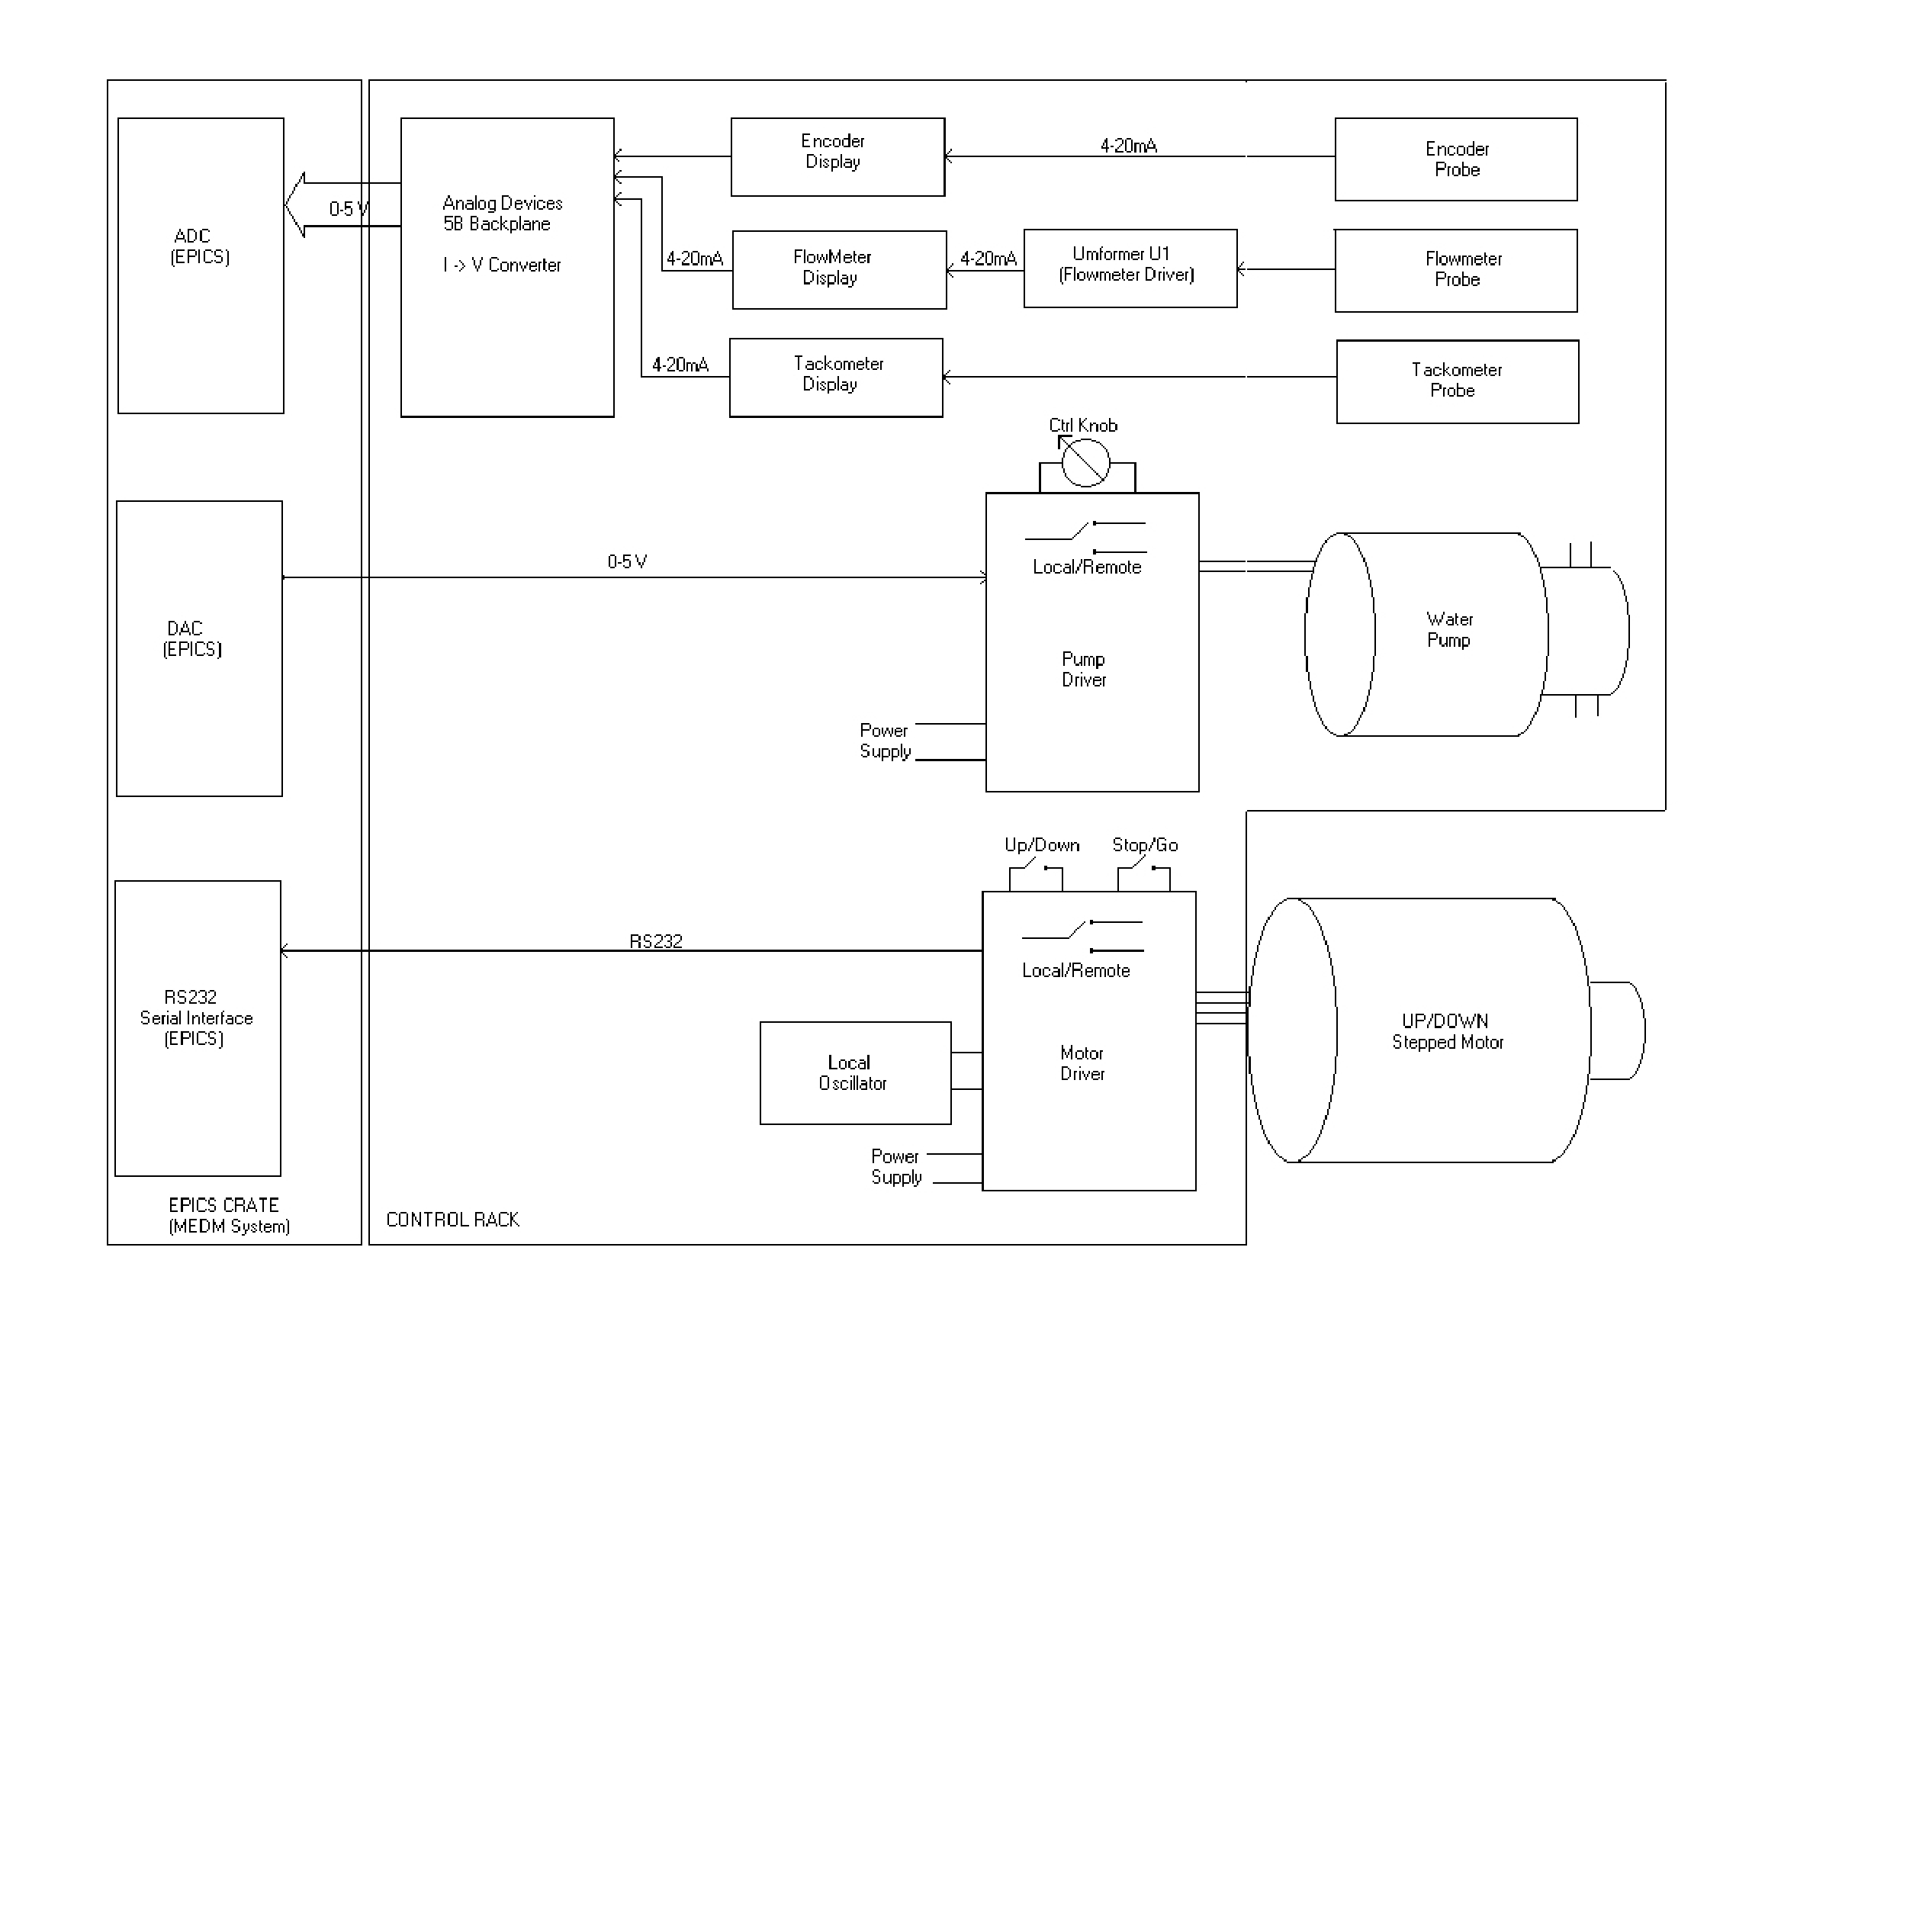
\includegraphics[width=0.9\textwidth]{wt2_glob}
  \end{center}
  \caption{Waterfall target: slow control system layout.}
  \label{fig:wt_fig1}
  \end{figure}

\infolevtwo{
  \begin{figure}
  \begin{center}
     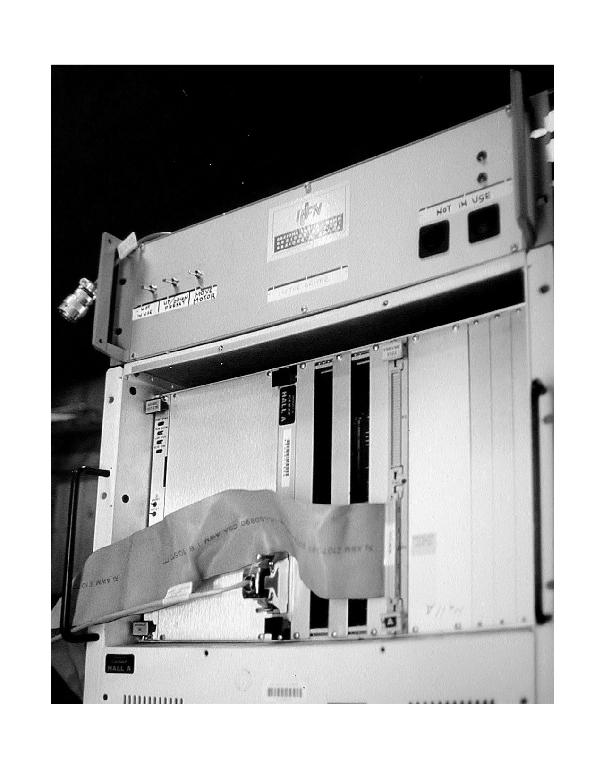
\includegraphics[height=0.4\textheight]{wt2_epics_crate}
  \end{center}
  \caption{Waterfall target: the EPICS Crate.}
  \label{fig:wt_crate}
  \end{figure}

  \begin{figure}
  \begin{center}
     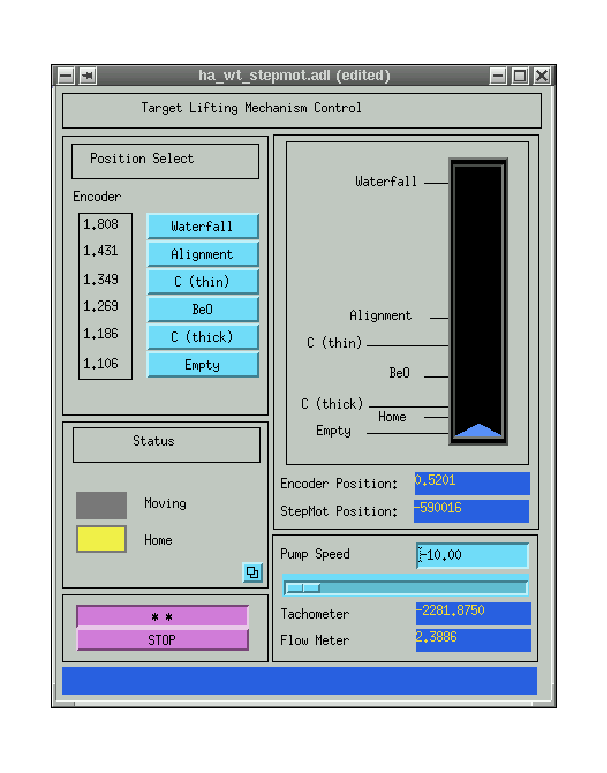
\includegraphics[  width=0.95\textwidth,height=0.60\textheight]{wt2_hawt-color}
  \end{center}
  \caption{Waterfall target control GUI.\label{fig:wt_GUI}.}
  \end{figure}

  \begin{figure}
  \begin{center}
    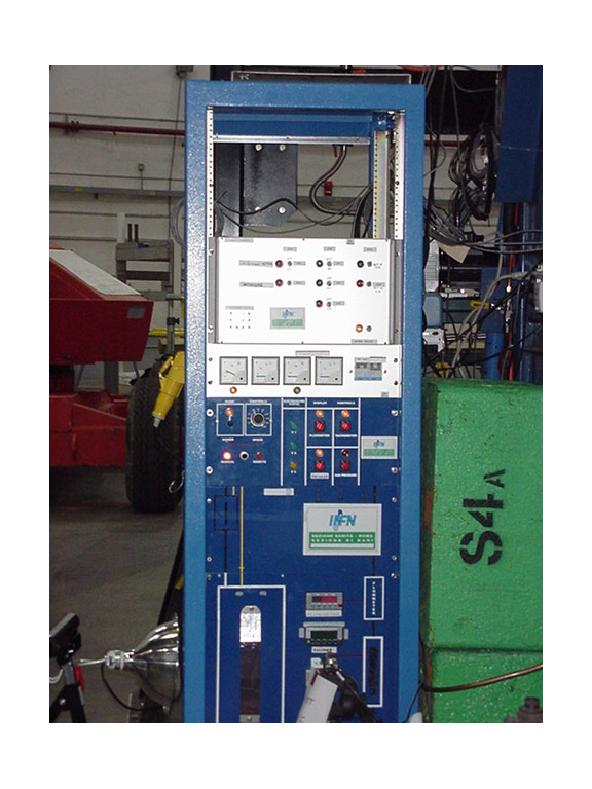
\includegraphics[  width=0.95\textwidth]{wt2_control-rack-color}
  \end{center}
  \caption{Waterfall target: control rack.\label{fig: wt_control rack}}
  \end{figure}
} %infolev


All of the analog signals coming from the transducers are to be read
by the ADC module, in the EPICS crate. For this reason, they are grouped
in a single cable, coming out of the rack, and connected to the the
ADC patch panel. These are slow signals: tachometer {[}arbitrary units{]},
flowmeter{[}l/min{]}, position encoder {[}arbitrary unit{]}, and do
not need a fast acquisition rate. The transducers, as indicated above,
all have 4-20~mA current output, for better noise immunity. The transducers
are located in the rack and send their signal to a current-to-voltage
converting board, located on the back side of the rack. This is called
5B Backplane, and contains 5B32 modules, which are insulated current
input and 4-20~mA to 0-5~V converters. Conversion to voltage is
necessary, to let the signals be acquired by the ADC of the MEDM system.
The pump command is a 0-5~V signal coming from the DAC module in
the EPICS crate.

The software control of the target is written in EPICS and run on
the IOC \mycomp{iochawt1}. The IOC uses serial communication, DAC
and ADC to control the target. The pump motor tachometer, flowmeter,
position encoder, and home switch are read through the ADC card. It
is common to have noise on the flowmeter, tachometer, and encoder.
The user should expect this noise and not be alarmed. The user should
check the camera on the control rack to make sure that the postion
encoder does indicate the proper target (there is some acceptable
slop on this number).

The motion control is achieved via a SHS - APS 3/A stepper motor controller.
Communication with this controller is achieved through a RS232 serial
connection. This controller counts absolute steps from the home postion.
The home postion is defined using the HOME routine on the expert page
of the GUI. Non-Experts are forbidden to use this function as serious
down time may result. If the target motion mechanism does not seem
to be moving to the selected target, execution of the HOME routine
might be needed and an expert must be called.

The pump speed control is achieved through a -5 - 5V DAC. The DAC
is 12 bit and negative voltages are not used in the application. Therefore
the minimum set postion for the pump speed is 2048. This corresponds
to 0V and 0 pump speed (pump is off). A setting of 4095 corresponds
to 5 volts and maximum pump speed. It is not possible to set the pump
speed outside these limits in software.

A counter readout (ITECO trading mod. 9210001) provides the tachometer
signal. The signal output from the module is 4-20~mA which is converted
to 0-5V and connected to the ADC. There is significant noise on the
ADC channel which seems to be a feature of the ADC. The user should
expect this noise and not be alarmed at oscillating values for the
tachometer signal.

The same counter readout is used for the flowmeter. The device is
read using the same ADC and thus, the signal has a similar level of
noise. The user should expect this noise and not be alarmed at oscillating
values for the flowmeter signal.

The postion encoder is the same type used on the collimators for both
arms. The encoder is displayed using a simple digital display on the
control rack. This display unit has a 4-20~mA output that is converted
to 0-5V and connected to the ADC. Again, the ADC value has significant
noise. The user should expect this noise and not be alarmed at oscillating
values for the encoder signal.


} %infolev
\infolevone{

\section{The Target Cell Windows}

A crucial component of the target is the cell window. Because it is
intended to employ beam current exceeding 50~$\mu $A, care must
be taken in choosing the window material, which otherwise could melt
from overheating. Consider the general case of a circular beam spot
and a circular target window, as illustrated in Fig.~\ref{fig:wt_curva}.
There is a continuous heat sink surrounding the window which is maintained
at temperature T$_{0}$ and located at a distance r$_{0}$ from the
center of the beam spot. The beam spot radius is r$_{1}$. The temperature
pattern which develops is characterized by two distinct regions. In
the logarithmic one the temperature is given by
\begin{figure}
\begin{center}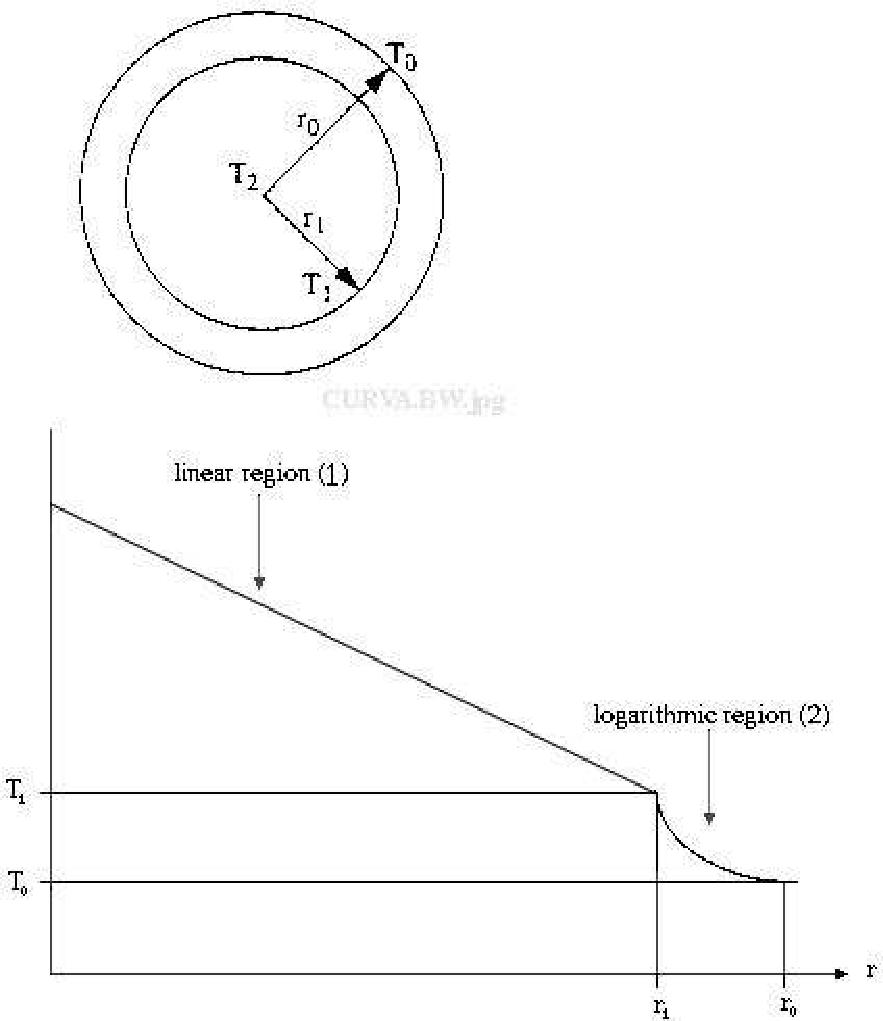
\includegraphics[width=0.4\textwidth]{wt2_curva_bw}\end{center}
\caption{Heat behavior of the beam entrance window.}
\label{fig:wt_curva}
\end{figure}

\begin{equation}
\Delta T_{1}=T_{1}-T_{0}=\frac{i\rho }{2\pi \kappa }\frac{dE}{dx}ln(\frac{r_{0}}{r_{1}})\end{equation}


while, in the linear region, the temperature is given by

\begin{equation}
\Delta T_{2}=T_{2}-T_{0}=\frac{i\rho }{4\pi \kappa }\frac{dE}{dx}\end{equation}


In both cases, \textit{i} is the beam current (in \textit{m}A, $\rho $
is the window material density, $\kappa $ is the thermal conductivity
and $\frac{dE}{dx}$ is the differential energy loss). The total temperature
rise above the surrounding heat sink temperature T$_{0}$ is thus

\begin{equation}
\Delta T=\Delta T_{1}+\Delta T_{2}=\frac{i\rho }{4\pi \kappa }\frac{dE}{dx}[1+2ln(\frac{r_{0}}{r_{1}})]\end{equation}


If a 100 $\mu $A beam of radius 25 $\mu $m and a window of radius
3 cm are considered (\textit{very} extreme situation), these are the
results for various materials:

\begin{center}\begin{tabular}{|c|c|c|c|c|c|}
\hline 
&
 $\rho $&
 $\frac{dE}{dx}$&
 $\kappa $&
 $T_{melt}$&
 $\Delta T$\\
 Material &
 ($\frac{g}{cm^{2}}$) &
 ($\frac{MeV}{\frac{g}{cm^{2}}}$) &
 ( $\frac{MeV^{0}C}{\mu A}$) &
 ($^{\circ }$C) &
 ($^{\circ }$C) \\
\hline
Al &
2.7 &
1.62 &
2.37 &
660 &
223 \\
\hline
Fe &
7.9 &
1.48 &
0.8 &
1530 &
1765 \\
\hline
Ti &
4.5 &
1.51 &
0.22 &
1660 &
3731 \\
\hline
Cu &
8.96 &
1.44 &
4.0&
1083 &
390 \\
\hline
Be &
1.85 &
1.61 &
2.1 &
1278 &
171 \\
\hline
W &
19.3 &
1.16 &
1.75 &
3410 &
1545 \\
\hline
Ta &
16.65 &
1.2 &
0.58 &
2996 &
4161  \\
\hline
\end{tabular}\end{center}

It is clear from the table that Be is the most suitable choice for
the entrance and exit windows. The window thicknesses vary for the
different targets used.

} %infolev
\infolevone{

\section{Target Layouts}

Three targets have been built: 

\begin{itemize}
\item a) the first one for the experiments E89-003 and E89-033 has got three
foils; 
\item b) the second one for the experiment E00-102 also has got three foils
but with some modifications; 
\item c) The third one for the experiment E94-107 has a single foil; 
\end{itemize}

\subsection{The Target for the Experiment E89-003 and E89-033}

Care was taken to optimize the foil configuration with respect to
the spectrometer acceptance and ejectile trajectory. A kinematical
overview of the target can be seen in Fig.~\ref{fig:wt_impact}, a cutaway
of the target in Fig.\ref{fig:wt_cell1}. The three foils are identical,
12 mm wide, and guided by poles which are 2 mm x 2 mm (Fig.~\ref{fig:wt_thfoil}).
In the direction normal to the target, the foils are separated by
22 mm. Along the target, the first foil is shifted down the page by
13 mm and second up the page by 13 mm. The foils are parallel, and
the angle between the beam direction and the direction normal to the
target is 30$^{0}$. The machining tolerance is less than 0.15 mm.

\begin{figure}
\begin{center}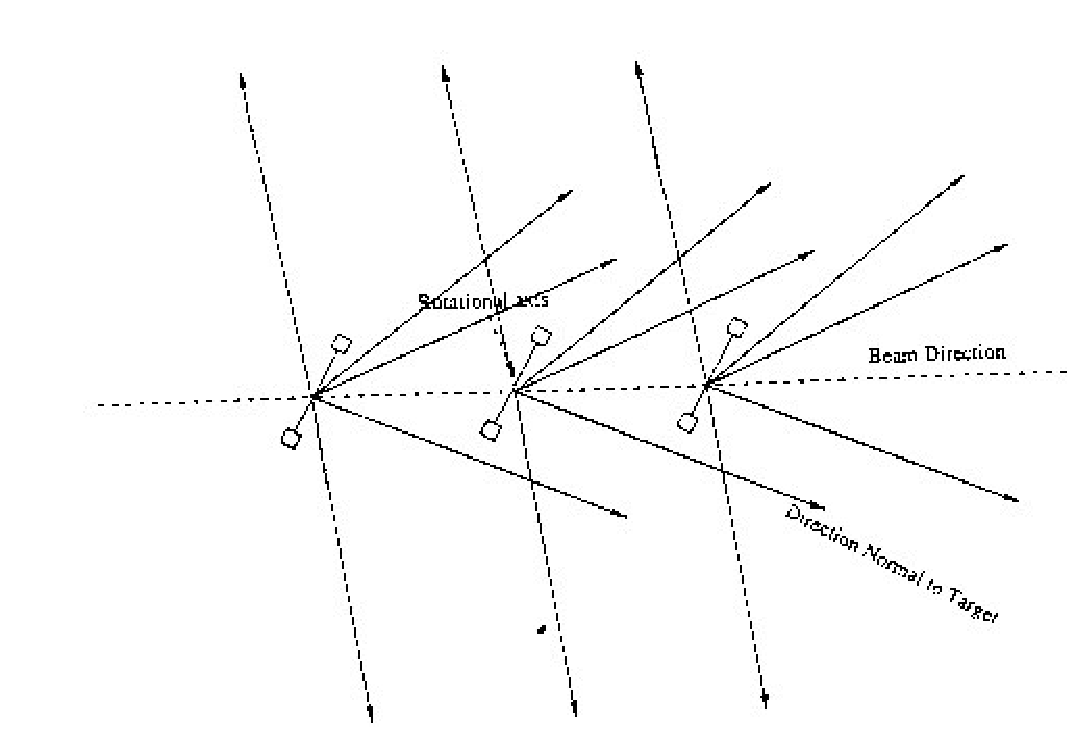
\includegraphics[  width=10cm]{wt2_impactschem}\end{center}
\caption{Preferential scattering angles for E89-003 and E89-033.}
\label{fig:wt_impact}
\end{figure}
\begin{figure}
\begin{center}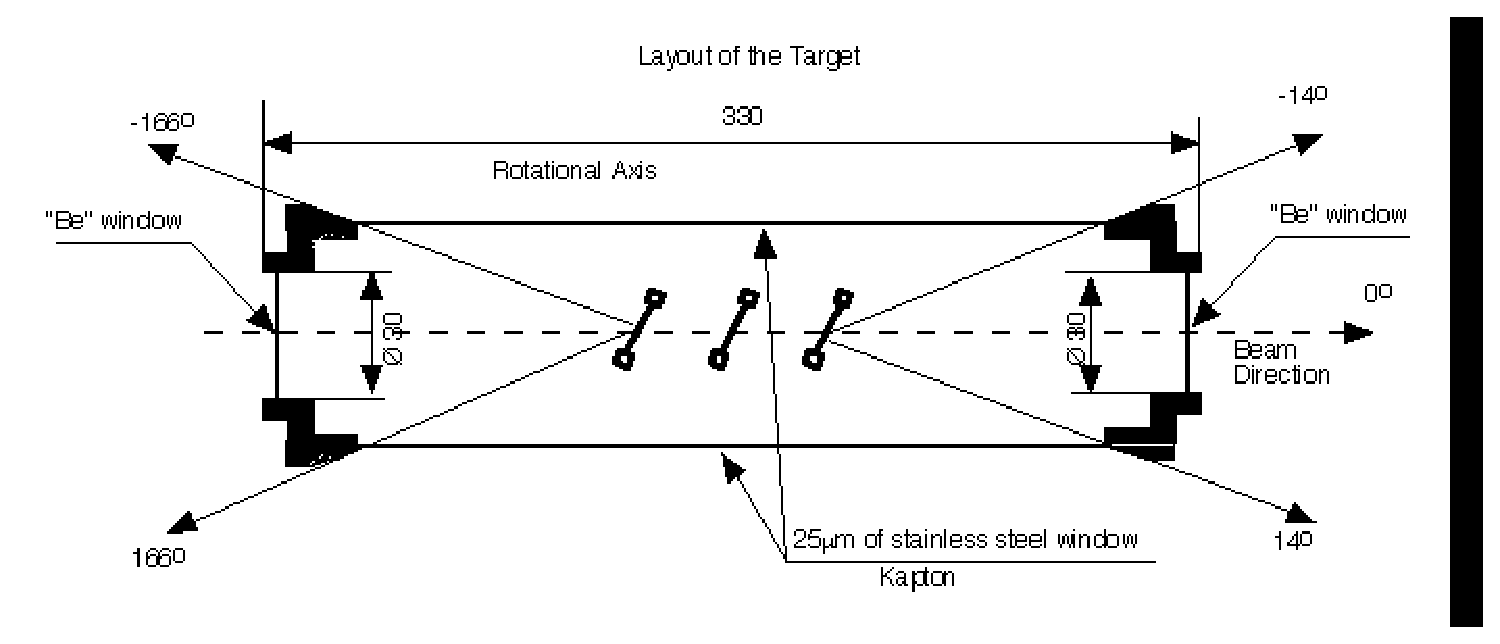
\includegraphics[  width=12cm]{wt2_cell1}\end{center}
\caption{A cutaway of the waterfall target cell used in E89-003 and E89-033.}
\label{fig:wt_cell1}
\end{figure}


\subsection{The Target for the Experiment E00-102}

This target has been modified for the experiment 00-102 to accommodate
the new kinematics (Fig.~\ref{fig:wt_oee-kin}). The concept is the same,
the geometry is slightly different, both for the target and for the
container.% (see drawings in the appendix). 
The Be window thickness
is 200 $\mu $m.
\begin{figure}
\begin{center}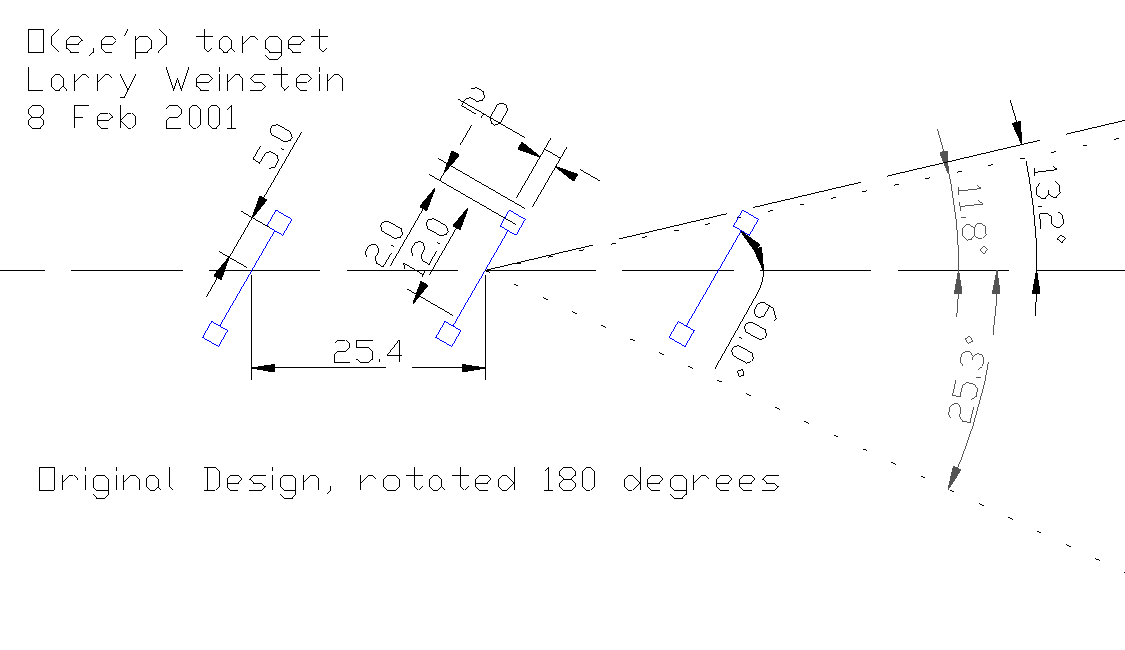
\includegraphics[  width=10cm]{wt2_oe-targ-unch}\end{center}
\caption{Preferential scattering angle of the target for the E00-102 experiment.}
\label{fig:wt_oee-kin}
\end{figure}



\subsection{The Target for the Experiment 94-107}

The E94-107 collaboration, in consultation with Hall A, has decided
to use a single foil one. The choice is driven by ease of construction,
minimization of software reconstruction for extended targets and improved
PID which is realized with the RICH. The missing mass resolution is
not significantly affected by this choice. The thickness of the Be
window has been increased (150 $\mu $m) because of the bigger diameter
of the downstream window.% The drawings are in the appendix. 

} %infolev

\infolevtwo{
\section{Operating Procedure}
\label{sec:oper_proc}

 There are two main points of operation, when using the system: the
first, to position the appropriate target in front of the beam, by
moving the target up or down, and the second one is, to control the
water pump. Both these operations can be done by using the GUI%
\infolevone{ (see Sec.\ref{sec:wt_slow_contr})}%
\infolevtwo{ (see Fig.\ref{fig:wt_GUI})}%
 accessable from the standard Hall A controls screen.
\begin{safetyen}{20}{15}
User operation of the target is achieved through this GUI only.
Any problems with the target must be addressed by an expert. A list
of experts is give in Table \ref{tab:wt_experts}.
The experts may perform some operations manually.
\end{safetyen}

The target consits of a positioning system that places one of 5 targets
(plus empty) on beam line and a water pump which circulates the target
fluid for the waterfall target. Under normal operations, the pump
should circulate $\sim 3$ l/min. 
\begin{safetyen}{20}{15}
A list of targets and maximum allowed
currents is given in Table~\ref{tab:target-list}. 
\end{safetyen}

\begin{table}[htp]
\begin{center}
\begin{tabular}{|c|c|c|}
\hline 
Target& Max Current& Max Current\\
      &Unrastered  & Rastered\\
\hline\hline 
$H_{2}O$         & 140 $\mu$A &   0 \\ \hline
Al alignment     &   0        &   0 \\ \hline
$^{12}C$ (thin)  &  10 $\mu$A &  50 $\mu$A \\ \hline
$BeO$            &  10 $\mu$A &  50 $\mu$A \\ \hline
$^{12}C$ (thick) &  10 $\mu$A &  50 $\mu$A \\ \hline
Empty            & -          &  -         \\ \hline
\end{tabular}
\end{center}
\caption[Waterfall target: maximum beam currents]{Target positions and maximum beam currents for the Hall A Waterfall
  Target stack. For increases in these current
  limits contact the Hall A run coordinator.}
\label{tab:target-list}
\end{table}

%\infolevlttwo{The detailed operation procedure is described in the
%  full version of OSP\cite{HallAosp}.}

As it has been mentioned in Sec.\ref{sec:wt_slow_contr}, it
is common to have noise on the ADC reading out the 
flowmeter, tachometer, and encoder.
The user should expect this noise and not be alarmed. 
The user operator should compare the displays on the GUI% 
\infolevtwo{~(Fig.\ref{fig:wt_GUI})} 
with the displays visible in the camera focused on the control rack.
In particular, one should make sure that the postion
encoder does indicate the proper target (there is some acceptable
slop on this number).
} %infolev
\infolevtwo{
\subsection{Startup of the system}

The startup and shutdown procedures require access to the equipment
inside Hall A.

\subsubsection{First startup of the System}

Before remote operation of the system can be used, the system must
be configured correctly. To do this, one has to perform the following
procedure with the waterfall control hardware (inside Hall A):

\begin{itemize}
\item Set the pump manual/remote switch to ``manual'' position;
also make sure the pump speed knob, in front of the rack, is set to
zero. 
\item Go to the motor chassis module and set B1 microswitch, there indicated,
to the ``manual'' position (that is the ``off''
position for the switch).
\item Go to the slow control rack, and turn the main 110~V switch to ``ON''.
\item Turn the pump control to on, and gently turn the pump speed knob clockwise.
Check the water circuit operation: 

\begin{itemize}
\item If they are off, switch on the displays ( FLOWMETER, TACHOMETER),
and check for proper operation.
\item If everything working correctly the pump control should be set to
the \char`\"{}remote\char`\"{} position. 
\end{itemize}
\item Check the positioning system:

\begin{itemize}
\item Switch the motor driver to ``manual'' mode. 
\item Go to the motor driver chassis and move the motor up and down by pressing
the switches on the front panel. 
\item Check that the motor is moving and make sure that the encoder display
is on, and working during the motor movement. 
\end{itemize}
\item If all components are operating correctly the system may be configured
for remote operation:

\begin{itemize}
\item Turn the main 110~V switch to ``OFF'', in front of
the slow control rack.
\item Settle the microswitch, on the back of the motor module, to ``ON''
(that is remote control position.)
\item Switch the 110V power supply to ``ON''.
\item Check the remote operation of the system in the counting room. The
procedure for remote operation is given in Sec \ref{sec:MEDM-operation}.
\end{itemize}
\end{itemize}

\subsection{System shutdown}

To shutdown the system one must take the following steps: 

\begin{itemize}
\item In Counting Room, set the pump speed to zero, and be sure the flowmeter
and tachometer indicate zero on their displays
\item Then go down to Hall A, turn the pump knob to zero and switch it off.
\item Finally, switch off the whole system by turning off the main 110VAC
switch, in front of the Rack.
\end{itemize}

\subsection{Troubleshooting}

\begin{itemize}
\item Emergency: Use of the system when the motor is broken \\
First of all, there is a spare motor in the shelf, ask the Hall A
maintenance technicians for details. \\
If for any reason, the motor can not be used, it is possible that
movement can be performed by using the crank, which is on top of the
target. To do this the crank must be put on the motor seat, and the
movement can be performed manually. If the encoder is working, one
can use the above table to positionsfor the targets, if the encoder
is unavailable, the microswitches put on top of the chamber will give
the correct alignment. \\
\begin{safetyen}{10}{10}
This procedure can be performed ONLY BY AUTHORIZED PERSONNEL, due
to the large vacuum load on the system and risk of possible free fall
when the motor is removed.
\end{safetyen}
\begin{safetyen}{0}{0}
\item Emergency: Use of the restore system, when motor has reached some
extreme position microswitch. \\
Due to the possibility of permanent damage to the system, this can
be done ONLY BY AUTHORIZED PERSONNEL. \\
\end{safetyen}
When a limit position is reached, an automatic control turns off the
power supply for the whole slow control system. In this case, a switch
is put in Hall A, near the slow control rack, which bypasses this
emergency stop and lets the operator move the motor in the correct
direction, bringing the system back to a more central position. This
has to be done manually, and visually checking the motor behavior,
because of the risk of damaging the target motion mechanism. Finally,
when done, the moving system has to be put back to the remote position,
and it has to be checked if this works well, or not. Fix the trouble
( a spare motor driver is in the shelf, if needed), and normal work
can begin again.
\end{itemize}

} %infolev

\infolevtwo{
\section{Standard Operations}
\label{sec:MEDM-operation}

These operations include moving the target ladder in order
to install the target needed and the water-pump
control. They should be performed using the GUI (Fig.~\ref{fig:wt_GUI}).
%All user aspects of the Hall A Waterfall Target are controlled through
%a single screen named {}``Target Lifting Mechanism Control'' (ha$\_$wt$\_$stepmot.adl).\\

\subsection{Target Selection}

The target postion is selected on the left side of the GUI under Position
Select. There are six options. The desired target is selected by clicking
on the particular target button. 
 Basically, this takes a present position and places it in the 
``set position'' input box. A specific position can also be entered 
directly into this box.
If the target is not already on the
desired postion, the user should see the ``moving'' LED turn yellow
in the Status display. The graphic display to the right of the selection
boxes should update; the blue diamond indicating the current postion
of the target. In addition, the ``Encoder Postion'' and ``StepMot
Postion'' displays to the right of the GUI should update indicating
the target is in motion. 
If the motor hits a
limit switch, the motion will stop and the ``Limits'' status will
indicate which limit is active. 

NOTE: the motor can be stopped at
anytime by pushing the purple button labeled ``STOP''. 

If the motion does not appear to be operating
correctly, call an expert. At the end of the motion sequence the encoder
postion should be close to the value in text next to the target button.
The value on the camera should be within $\pm 0.0030$ on the encoder
readout. If this is not the case call an expert. 

Note that any target
motion will trip and FSD. The MCC should be informed of all target
motion. If for some reason during the target motion there is a need
to stop, click on the stop button. Motion can be restarted by selecting
another target.

There is an access from the ``Status'' section to an expert screen.
Only experts should use the functions on this screen there are no
user features here.

In addition to the camera on the control rack, there is a camera on
top of the pivot focused on the motion mechanism. The target postions
and names are labled in a visible fashion. The user should double
check this camera as well to make sure the motion mechanism is behaving
as expected.

Finally, there are micro-switches that provide an FSD signal when
not on a target. If for some reason an FSD is still tripped after
a move to a new target, an expert should be called.


\subsection{Pump Speed Control}

The pump speed control is set using the slider bar or input field
in the {}``Pump Speed'' section. This input may range from 2048
to 4096 corresponding to a 12 bit DAC 0-5V output. The output of the
DAC is converted to 4-20 mA and used to control the pump speed. An
input of 2048 (0V) will stop the pump. An output of 4095 (5V) sets
the pump speed at $\sim 1800$ on the display which is roughly 6 l/min.
This should be more than adequate for normal operations. If the pump
does not function properly or more flow is desired, an expert must
be called. The tachometer and flowmeter displays should always be
checked with the displays on the camera.


\subsection{Rebooting the IOC}

The name of the IOC is iochawt1. The IOC may be rebooted by logging
into the IOC via telnet and typing reboot. If this is not possible,
(i.e. the IOC is not responding to remote login) call an expert.
} %infolev

\infolevtwo{

\section{Troubleshooting (Experts only)}

This section is intended as a reference for experts only. 
\infolevfour{
  Figure \ref{fig: wt_control rack} shows the control rack. 
  Figure \ref{fig: wt_IOC-rack} shows the IOC rack.
}%infolev
\begin{figure}
\begin{center}
  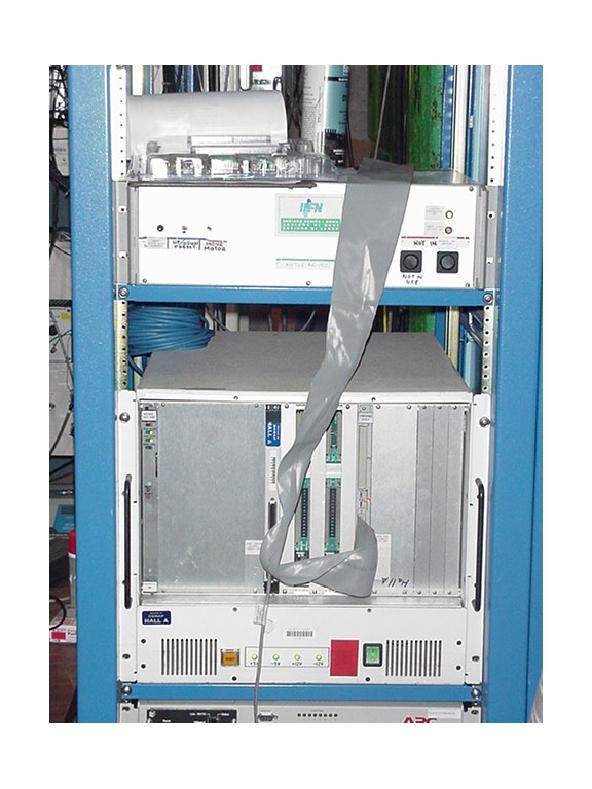
\includegraphics[  width=0.90\textwidth]{wt2_IOC-rack}
\end{center}
\caption{IOC rack for waterfall target.\label{fig: wt_IOC-rack}}
\end{figure}

\subsection{Manual motion operation (Experts only)\label{sec: wt-Manual}}

Ensure that the motor controller power is off. The power may be turned
off at the front of the main control rack under the beam line. In
the motor control rack located next to the IOC, there is a small chassis
mounted box. At the back of the box, there is a DIP switch clearly
marked with black pen labled B1. This switch must be set to OFF to
put the controller in manual mode. Restore power from the control
rack under the beam line. Return to the motor control box. If the
green LED at the right of the box turns on, all is well and the target
can be moved up or down by setting the direction switch and toggling
the move switch. To restore the remote operation of the system cut
power at the main control rack under the beam line. Return the B1
DIP switch to ON and restore power to the system. At this point the
controller does not {}``know'' where it is. The HOME routine must
now be run. See Section \ref{sec: wt-HOME} for proper use of the HOME
routine.


\subsection{Use of the HOME routine\label{sec: wt-HOME}}

Use of the HOME routine can be effected from them the main control
GUI. In the {}``Status'' section of the GUI, there is a small button
that brings up the expert page. Be sure that the physical position
of the target is a few centimeters above the H2O target. This can
be seen at the top of the scattering chamber. The HOME routine will
not properly execute from the H2O target postion. The target might
have to be moved manually above the H2O target postion (see Section
\ref{sec: wt-Manual}). Press the HOME button. The target should move
in the direction of the HOME switch which is located near the empty
target position. If the target does not move in the correct direction,
move the target manually to some position close the the BeO target
position. This may take some time. The motor controller will look
for the HOME switch by moving the system up. When the HOME switch
is activated, the target will start moving down; when it finds the
HOME switch again it will stop. This ensures that the HOME position
is not affected by the hysteresis in the switch.


\subsection{Hardware limit over travel}

If a limit switch (either upper or lower) is tripped, the target motion
control system will lose power. This is designed so that the lifting
mechanism will not be damaged. In this case, the limit must be bypassed
and the target moved off of the limit manually. First, the controller
must be set to manual mode. See Section \ref{sec: wt-Manual}. At the
front of the box, there is a switch labled bypass power. Turn this
switch down; the yellow LED above should turn on. Also on the front
of the box is limit switch bypass button. Press this button and move
the target manually. BE SURE TO MOVE IN THE CORRECT DIRECTION; severe
damage to the system may result from improper use of this feature.
If the motor does not seem to be moving, page Dave Meekins or Scot
Spiegel. As the power has been cycled to this module, it is now necessary
to run the home routine (see Section \ref{sec: wt-HOME}). Disable bypass
power when finnished with motor reset.


\subsection{Manual water pump operation}

Operation of the water pump in the manual mode is simple. There is
a switch at the front of the main control rack (located under the
beam line) that can be toggled to remote or manual operation. The
pump power switch must be on for the pump to work. The pump speed
is controlled via the knob which can be rotated clockwise for more
speed. Please do not run the pump faster than 2000 as shown on the
tachometer display. This causes undue strain on the system.

} %infolev

\begin{safetyen}{0}{0}
\section{Safety Assessments}
\end{safetyen}

\begin{safetyen}{50}{50}
The water fall target system is much more simple than the standard
target configuration for Hall A. There are therfore fewer hazards
which need to be addressed. The target does use the standard Hall~A 
scattering chamber for experiment E00-102. The safety hazards for
the scatting chamber have been addressed in the standard Hall A safety
documentation (see Chapter.~\ref{sec:target_chamb}% 
\infolevone{ and Sec.\ref{sec:cryo_targ_cmb_falure}}). 
The following subsections outline the potential hazards
and how each must be addressed.
\end{safetyen}

\infolevone{
\begin{safetyen}{10}{10}
\subsection{Radiological hazards}
\end{safetyen}

Due to the large beam currents required for the referenced experiments,
the potential for radiological contamination of the target fluid and
scattering chamber area exists. Therefore, all personnel entering
the target area after beam has been impinging on the target must follow
standard radiological control procedures. Prior to entry into the
area the Radiation Control Group must be consulted. The system must
only be accessed by authorized personnel


\begin{safetyen}{10}{10}
\subsection{The electrical power and slow control systems}
\end{safetyen}

The system is supplied by 110~V AC voltage. All the lines at these
voltages are kept inside the rack, and the plugs satisfy the European
CE rules for these voltages. The supplies for the single diagnostic
and control devices are inside the rack are all at 5~V DC, 12~V
DC, 24~V DC. The pump requires 110~V DC. The Motor Driver needs
a special 80~V DC voltage. A custom power supply unit has been built
for this purpose, and this unit is kept in the so called 
``Power Supply Unit'' at the top of the rack, together with the other
supply units. 

The signal lines are low voltage (no higher than 12~V DC the digital
lines, 0-5~V or 4-20~mA loops) and kept separated from the supply
lines by using different connectors and separated cables. Isolated
input lines have been used for the analog lines. A potential hazard
outside of the rack, are the motor cables, which may be handled only
by AUTHORIZED PERSONNEL and with the motor power supply switched off.
An 80~V DC/2A (square wave, duty cycle 0,5) current flows in these
cables when the motors are in standby mode. This current reaches up
to 7~A (square wave, duty cycle 0,5) when motors are moving. These
high power lines are kept separated from the low voltage lines in
all cases. The pump power supply line is kept inside the rack, and
in a position that cannot be reached unless the side panel of the
rack is opened.

Access to the rack is controlled by appropriate signage indicating
the hazard and list of personnel authorized access.


\begin{safetyen}{10}{10}
\subsection{The water system}
\end{safetyen}

There are about 17 liters of pure water in the circuit. The water
tank, the tubes, the target and the cell containing the target fluid
are made of stainless steel. Connections between individual parts
of the system have been made with \char`\"{}swagelok\char`\"{} connectors.
The system has been leak checked with gas up to 2 bars. No water leakage
is expected except in case of breaking of the windows of the target
cell. In this case, some water carrying some radioactivity may leak
into the scattering chamber (which is a contained environment). The
calculations performed by Geoff Stapleton show that
the radiological precautions necessary are rather low. The water should
not be released into the hall drains. Measurements at convenient intervals
will be made by the radiation control group on samples to permit determinations
of the radionuclide yields. In the case of water loss or the need
to drain the water, the radiation control group has to be informed
to permit precautionary measurements and controls. Appropriate sinage
on the water system indicates this.

\begin{safetyen}{10}{10}
\subsection{Thin windows on the target cell}
\end{safetyen}

The beam passes through two windows, which are made of Be (203 $\mu $m
thickness). It has been calculated (using the FNL-1380 Thin Window
Vacuum Vessel Guide from Fermilab) that the Be windows will have a
safety factor of 3 beyond the 1/2 yield requirement listed in the
Fermilab document. It has therefore been concluded that the windows
are adequate for use on this target cell.

The two scattering windows are made of kapton except for experiment
E00-102 where the scattering windows are made from 25 $\mu $m thick
stainless steel shim stock (SST 302; Hardness: 40-45 RC; Tensile Strength:
185000 psi). Three of these scattering windows have been hydro-tested
and in each case the window did not fail until slightly above 3 times
over pressure (50 psig or higher). A summary of the test results is
shown in Table \ref{tab: window-table}. It is important to note that
the windows only have a 1 atm load on them when the scattering chamber
is under vacuum. In this case, the windows are not accessable and
present no hazard to personnel.

%
\begin{table}
\begin{center}\begin{tabular}{|c|c|c|p{2in}|}
\hline 
Pressure&
\multicolumn{1}{c|}{Deflection}&
\multicolumn{1}{c|}{Deflection}&
\multicolumn{1}{p{2in}|}{Deflection}\\
(psig)&
\multicolumn{1}{c|}{Window 1}&
Widow 2&
Window 3\\
\hline
\hline 
0&
0&
0&
0\\
\hline
5&
53&
69&
55\\
\hline
10&
71&
85&
72\\
\hline
15&
82&
93&
82\\
\hline
20&
94&
111&
93\\
\hline
25&
104&
117&
103\\
\hline
30&
113&
128&
113\\
\hline
35&
124&
136&
122\\
\hline
40&
135&
141&
128\\
\hline
45&
143&
150&
-\\
\hline
50&
Failed&
160&
-\\
\hline
55&
-&
Failed&
Failed\\
\hline
\end{tabular}\end{center}
\caption[Summary of thin scattering window hydro-tests]%
{Summary of thin scattering window hydro-tests. Deflections are given
in (in$\times $1000). The scattering windows are made from 25 $\mu $m
thick stainless steel shim stock (SST 302; Hardness: 40-45 RC; Tensile
Strength: 185000 psi). \label{tab: window-table}}
\end{table}



\begin{safetyen}{10}{10}
\subsection{The slow control system}
\end{safetyen}

Due to the low voltages and little currents, there are no significant
hazards in working on the small signals; however, one must switch
the power off to the whole system before beginning to operate on it.
ONLY AUTHORIZED PERSONNEL may touch the signal lines using appropriate
lockout tagout procedures.


\begin{safetyen}{10}{10}
\subsection{The mechanical system}
\end{safetyen}

There are no hazards in handling the system when it is not in motion.
When the system is in motion one has to beware of the cog-wheels movements,
and keep hands and loose clothing away from the moving parts. For
this reason, it is FORBIDDEN to touch the system when it is in motion.
Additionally, the potential exists for remote operation of the motion
mechanism while it is being serviced. Therefore, to service the system
while it is installed, the appropriate lockout tagout procedures are
necessary. Signage stating this will be posted on the motion mechanism
upon installation in the hall.
} %infolev
\newpage
\begin{safetyen}{10}{15}
\section{Authorized  Personnel}
\end{safetyen}

\begin{namestab}{tab:wt_experts}{Waterfall target: authorized personnel}{%
   Waterfall target: authorized personnel}
   \namestabheader{Physicists}
   \DaveMeekins{\em Target Group}
   \MaurizioLucentini{}
   \namestabheader{Hall A Technicians}
   \EdFolts{}
   \RustySalmons{}
   \ScotSpiegel{}
   \MarkStevens{}
   \GaryDezern{}
\end{namestab}


% ===========  CVS info
% $Header: /group/halla/analysis/cvs/tex/osp/src/targets/waterfall-target.tex,v 1.6 2003/12/13 06:23:39 gen Exp $
% $Id: waterfall-target.tex,v 1.6 2003/12/13 06:23:39 gen Exp $
% $Author: gen $
% $Date: 2003/12/13 06:23:39 $
% $Name:  $
% $Locker:  $
% $Log: waterfall-target.tex,v $
% Revision 1.6  2003/12/13 06:23:39  gen
% Septum added. Name tables. Polishing
%
% Revision 1.5  2003/12/05 07:35:03  gen
% WT2 modified. Polishing
%
% Revision 1.4  2003/11/21 18:13:11  gen
% waterfall-target and waterfall-safety combined
%
% Revision 1.3  2003/11/19 22:45:21  lerose
% eliminated extra figures
%
% Revision 1.2  2003/11/18 07:46:27  gen
% waterfall docs collection
%
% Revision 1.1  2003/06/06 17:09:04  gen
% Revision printout changed
%
% Revision 1.2  2003/06/05 23:30:01  gen
% Revision ID is printed in TeX
%
% Revision 1.1.1.1  2003/06/05 17:28:27  gen
% Imported from /home/gen/tex/OSP
%
%  Revision parameters to appear on the output

